\chapter{Our results}

In this chapter we are going to present our results. First some remarks about resolution and convergence of the shape within Auriga simulations for DM and MHD. Then we study the radial and historic profiles of DM and MHD halos, where we obtain the expected tendence found by Vera-Ciro et al. 2011. Then present our principal results, which are the ones referring the comparison DM-MHD.

\section{Analysis of convergence}
One of the principal factors that may bias our study is the resolution of the simulations we work with. This is an indicator principally thought to analyze the numerical convergence of the methods used to solve the non-linear equations for matter, and give validity over the output results overall. However, resolution may also directly affect our procedure for calculating halo shapes through the reduction of particles taken into account to calculate the inertia tensor.\\

To illustrate this, in figures \ref{fig:goodConvergenceDM,fig:goodConvergenceMHD} we compare the obtained halo shape at redshift 0 on level 3 and level 4 simulations for a halo in which resolution does not noticeably affect the results. In this case, we can say that there is good convergence of the studied quantities with very small numerical bias. However, this is not the case every simulated halo as they do not evolve similarly and some resolution-sensitive events may influence their history of formation. In this sense, in figures \ref{fig:badConvergenceDM,fig:badConvergenceMHD} we present one of the halos where resolution played the most appreciable role affecting the shape. In this case, although the difference is not extreme, it requires attention and a more careful analysis.\\

For instance, by simple inspection, we notice that there is no apparent systematic way in which resolution affects the halo shape. That is, sometimes the halo appears rounder and some times it is affected towards a more triaxial shape. This is important for our study as we focus our efforts on the analysis of the halo triaxial properties. Incidentally, it is also notable that, even for the case of good convergence, there is still a remaining difference of shapes in the MHD simulations. This means that the effect of resolution is stronger for gas than for DM.  


\begin{figure}[!ht]
  \centering
  \subfloat[halo 6 MHD]{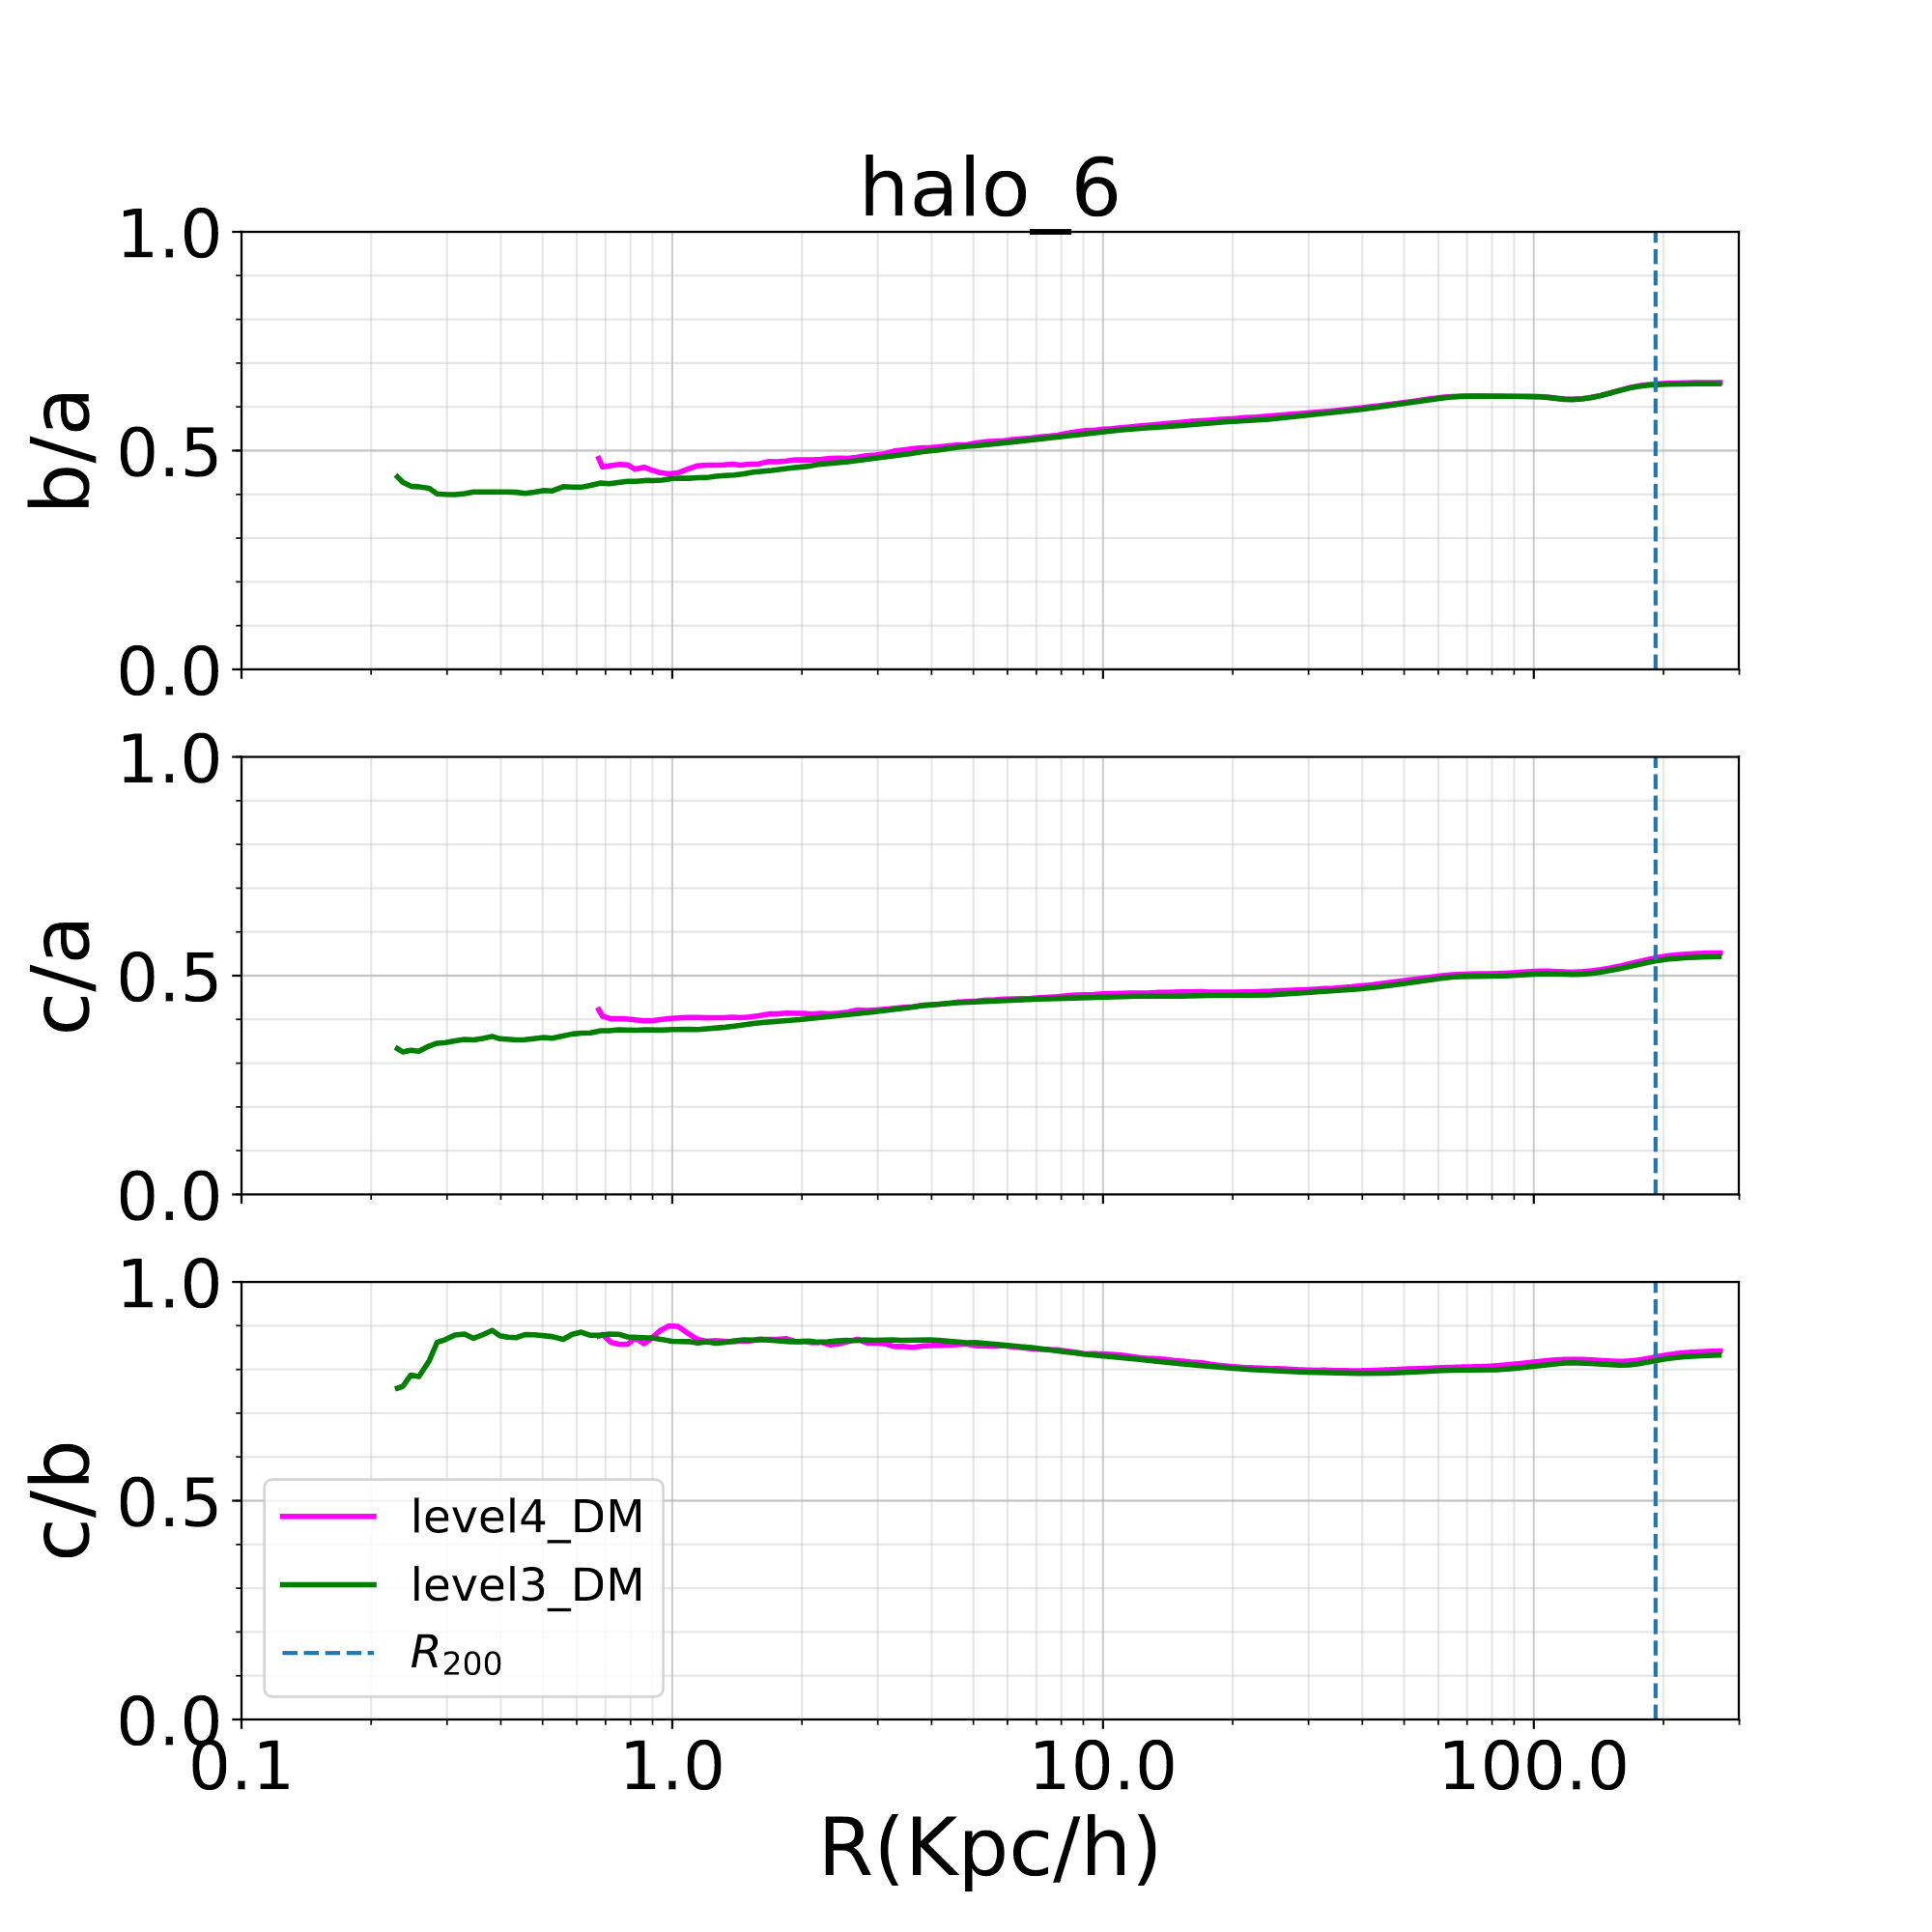
\includegraphics[width=0.5\columnwidth]{./pics/Convergence/halo6_DM_3Vs4_good.png}\label{fig:goodConvergenceDM}}
  \hfill
  \subfloat[halo 27 DM]{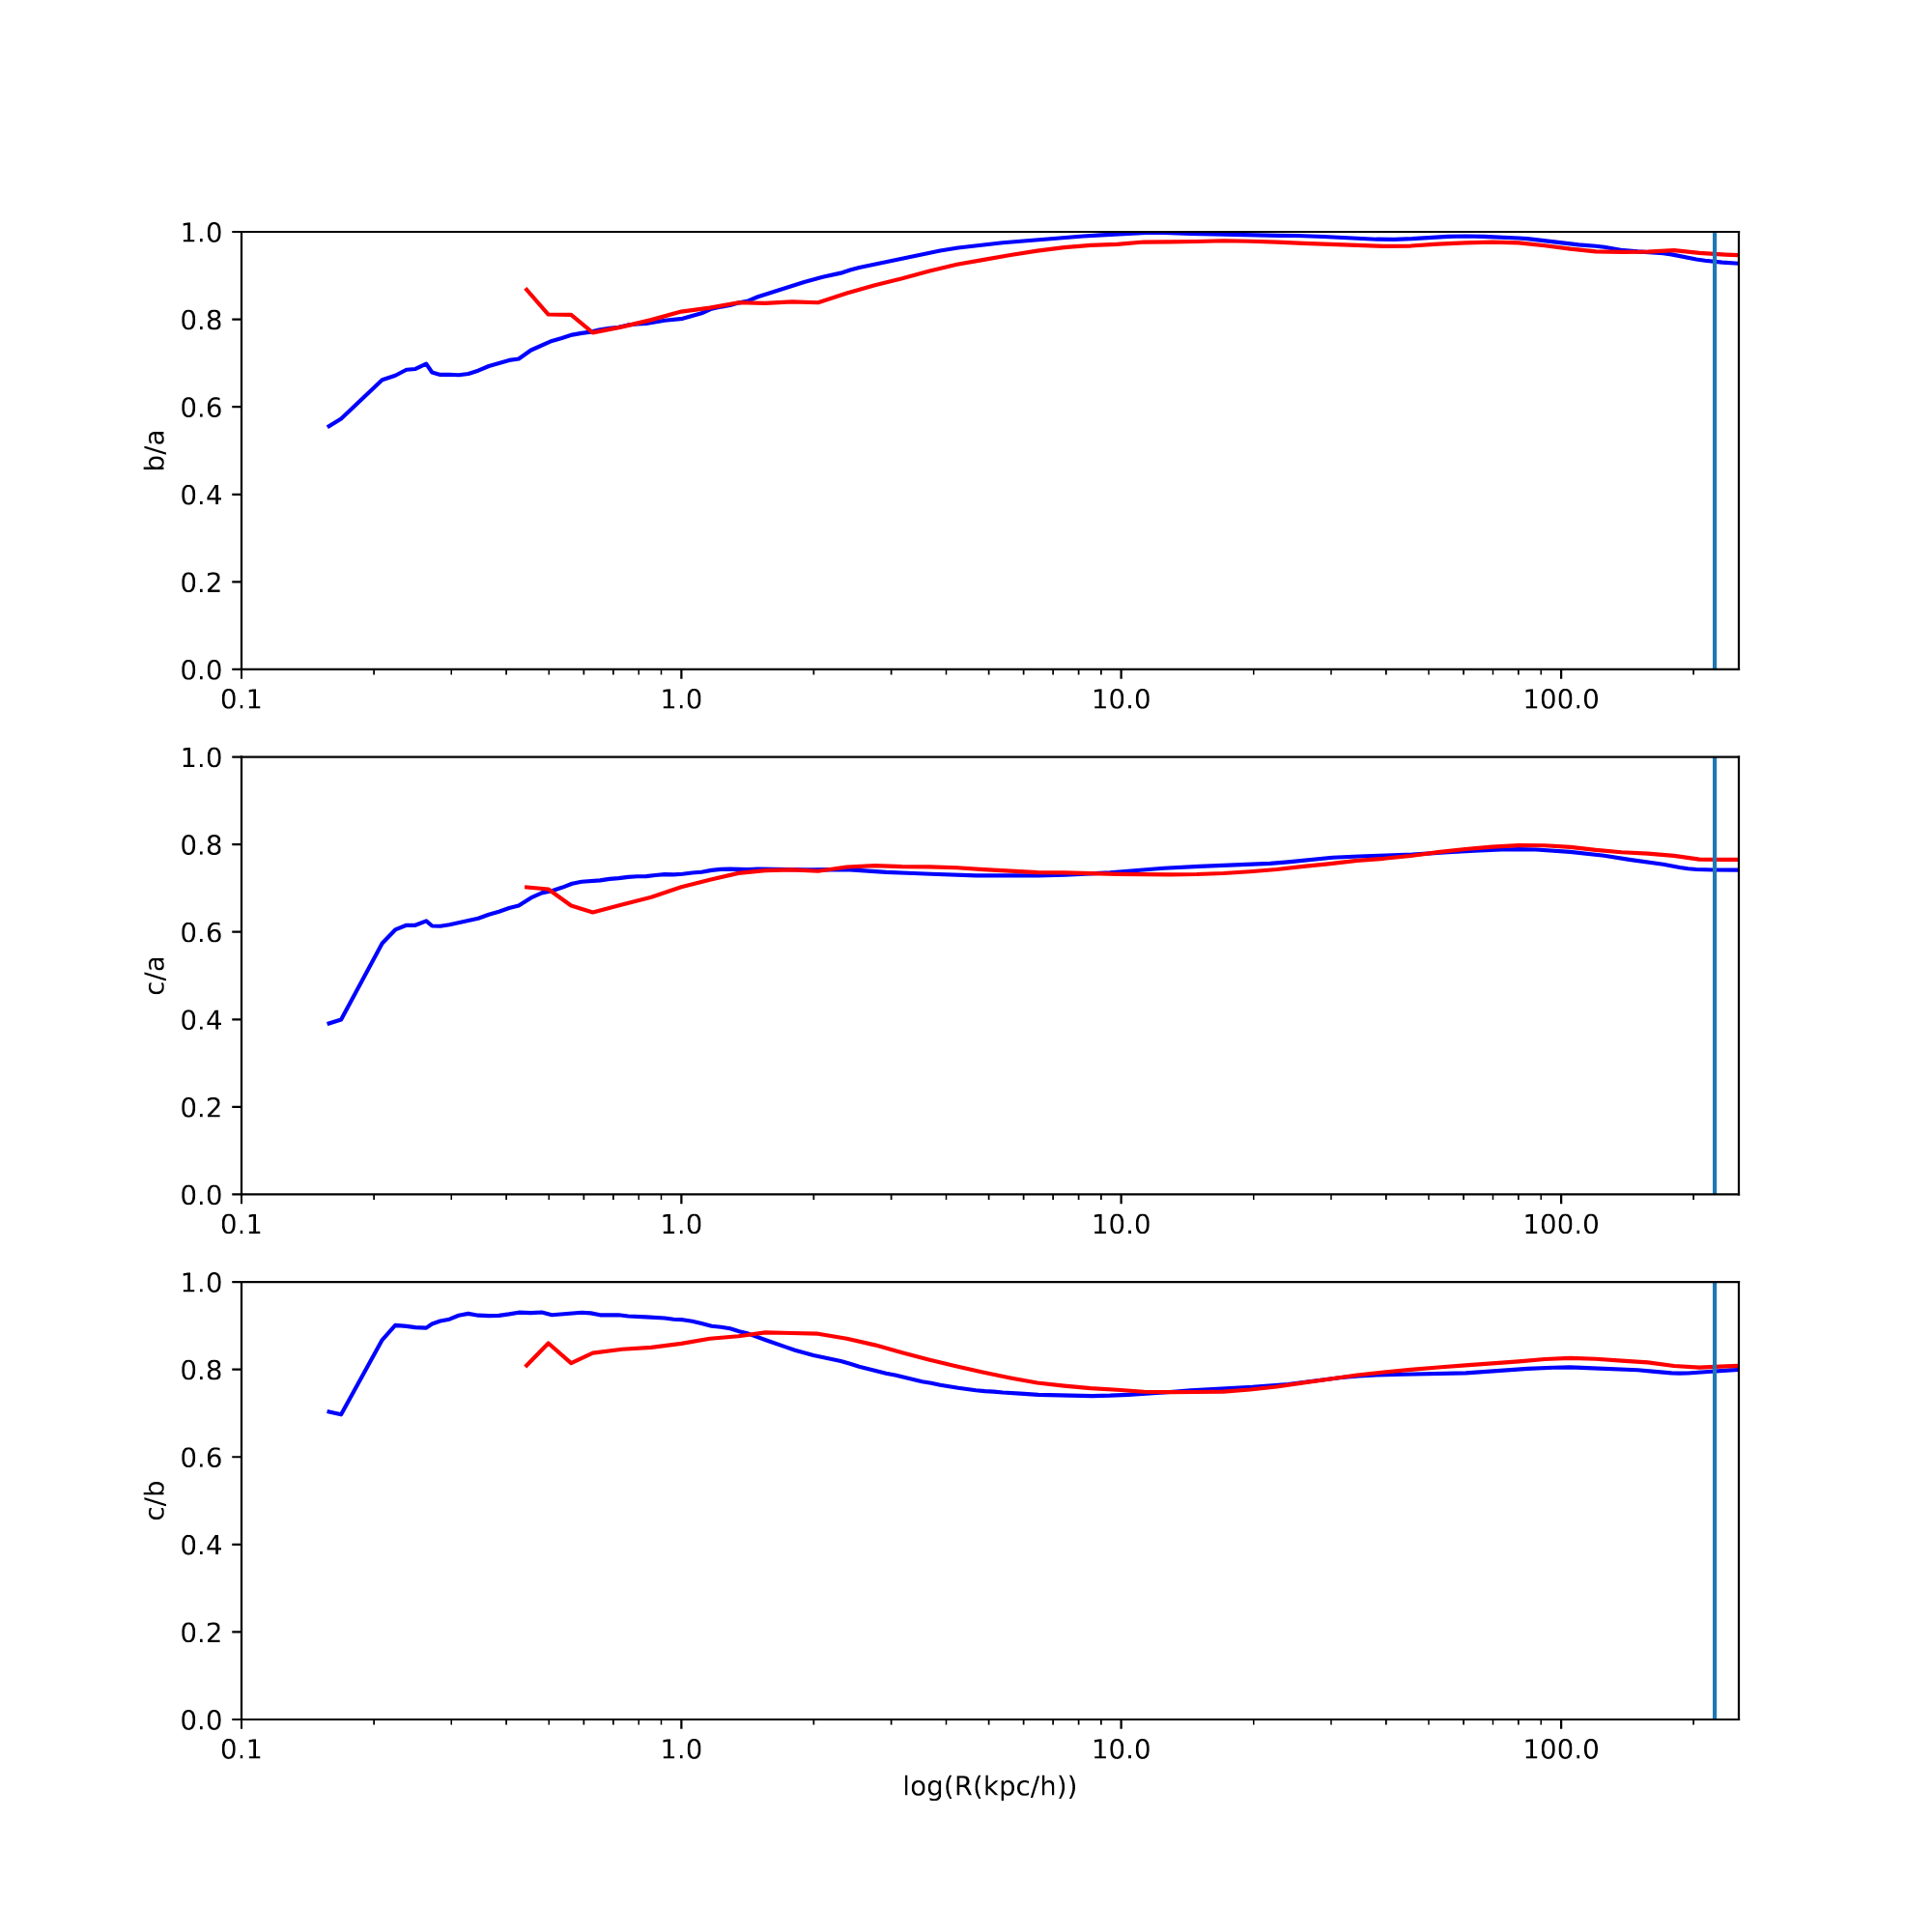
\includegraphics[width=0.5\columnwidth]{./pics/Convergence/halo27_MHD_3Vs4_good.png}\label{fig:goodConvergenceMHD}}
  \caption{Examples of halos where resolution did not have an appreciable effect on the halo shape. Level 3 (blue) and level 4 (red) calculations are in good agreement. \textbf{put labels, bigger axes font, add title} }
\end{figure}



\begin{figure}[!ht]
  \centering
  \subfloat[halo_21 MHD]{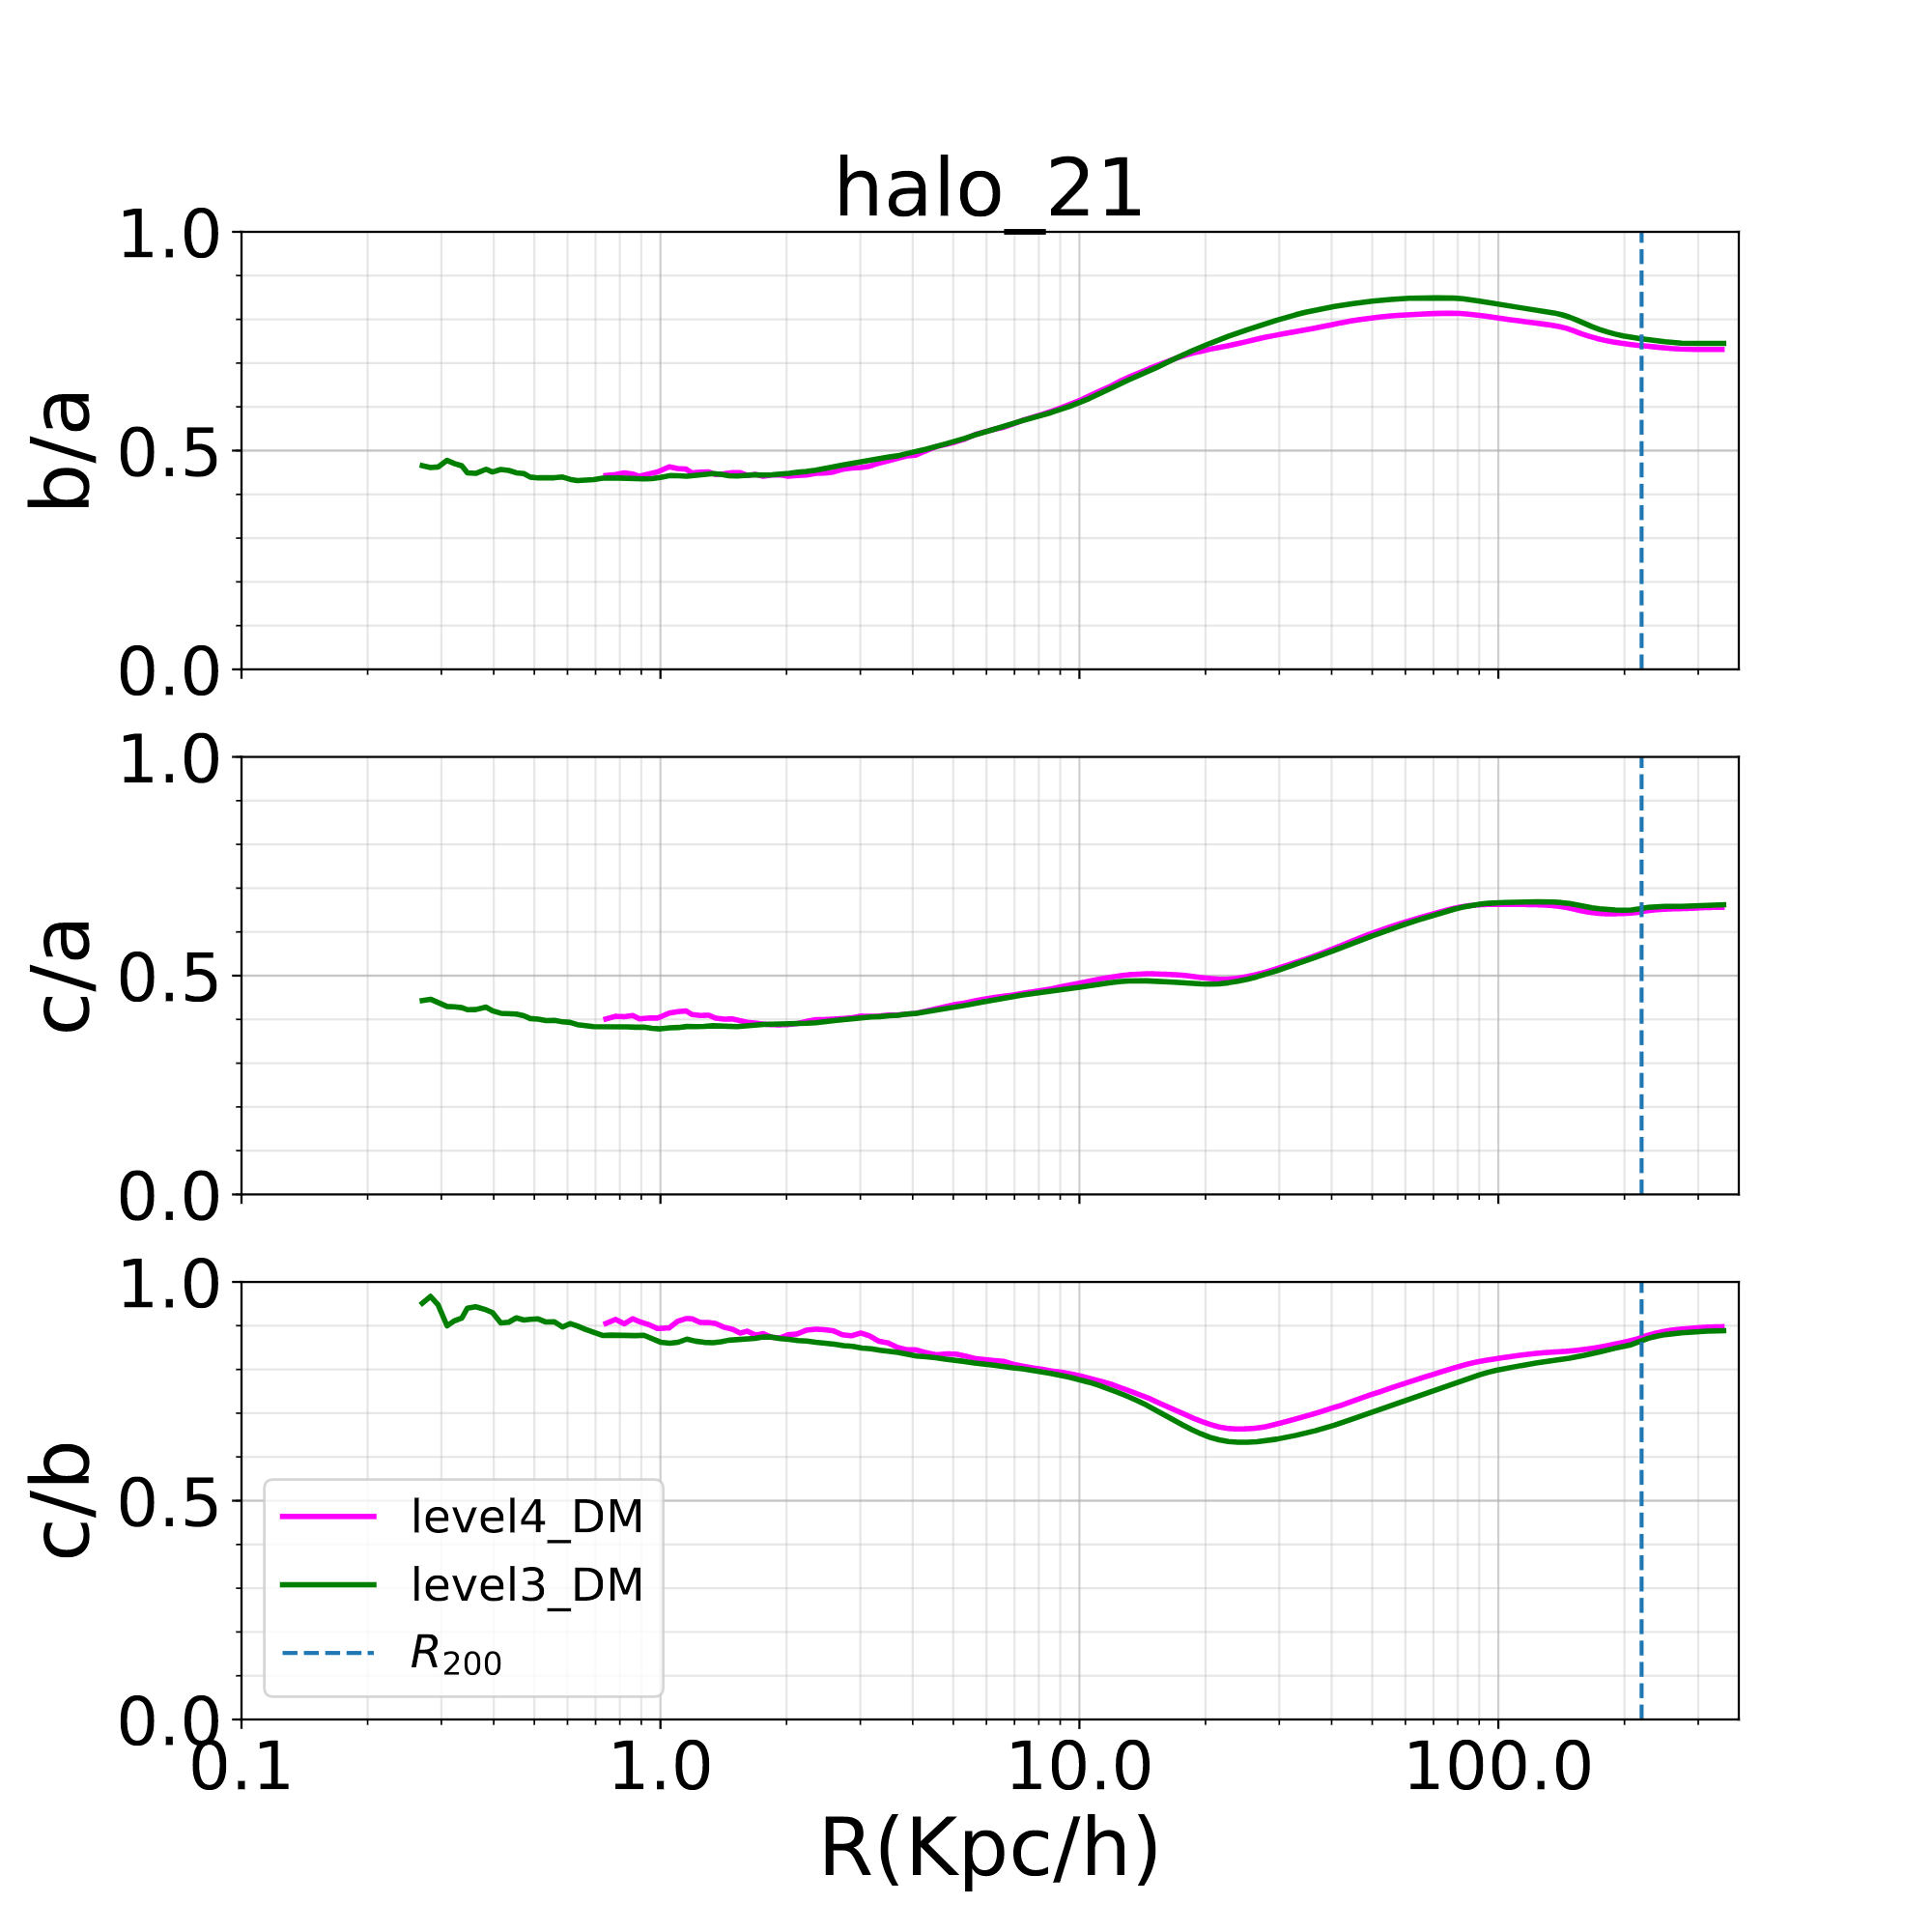
\includegraphics[width=0.5\columnwidth]{./pics/Convergence/halo21_DM_3Vs4_bad.png}\label{fig:badConvergenceDM}}
  \hfill
  \subfloat[halo_23 DM]{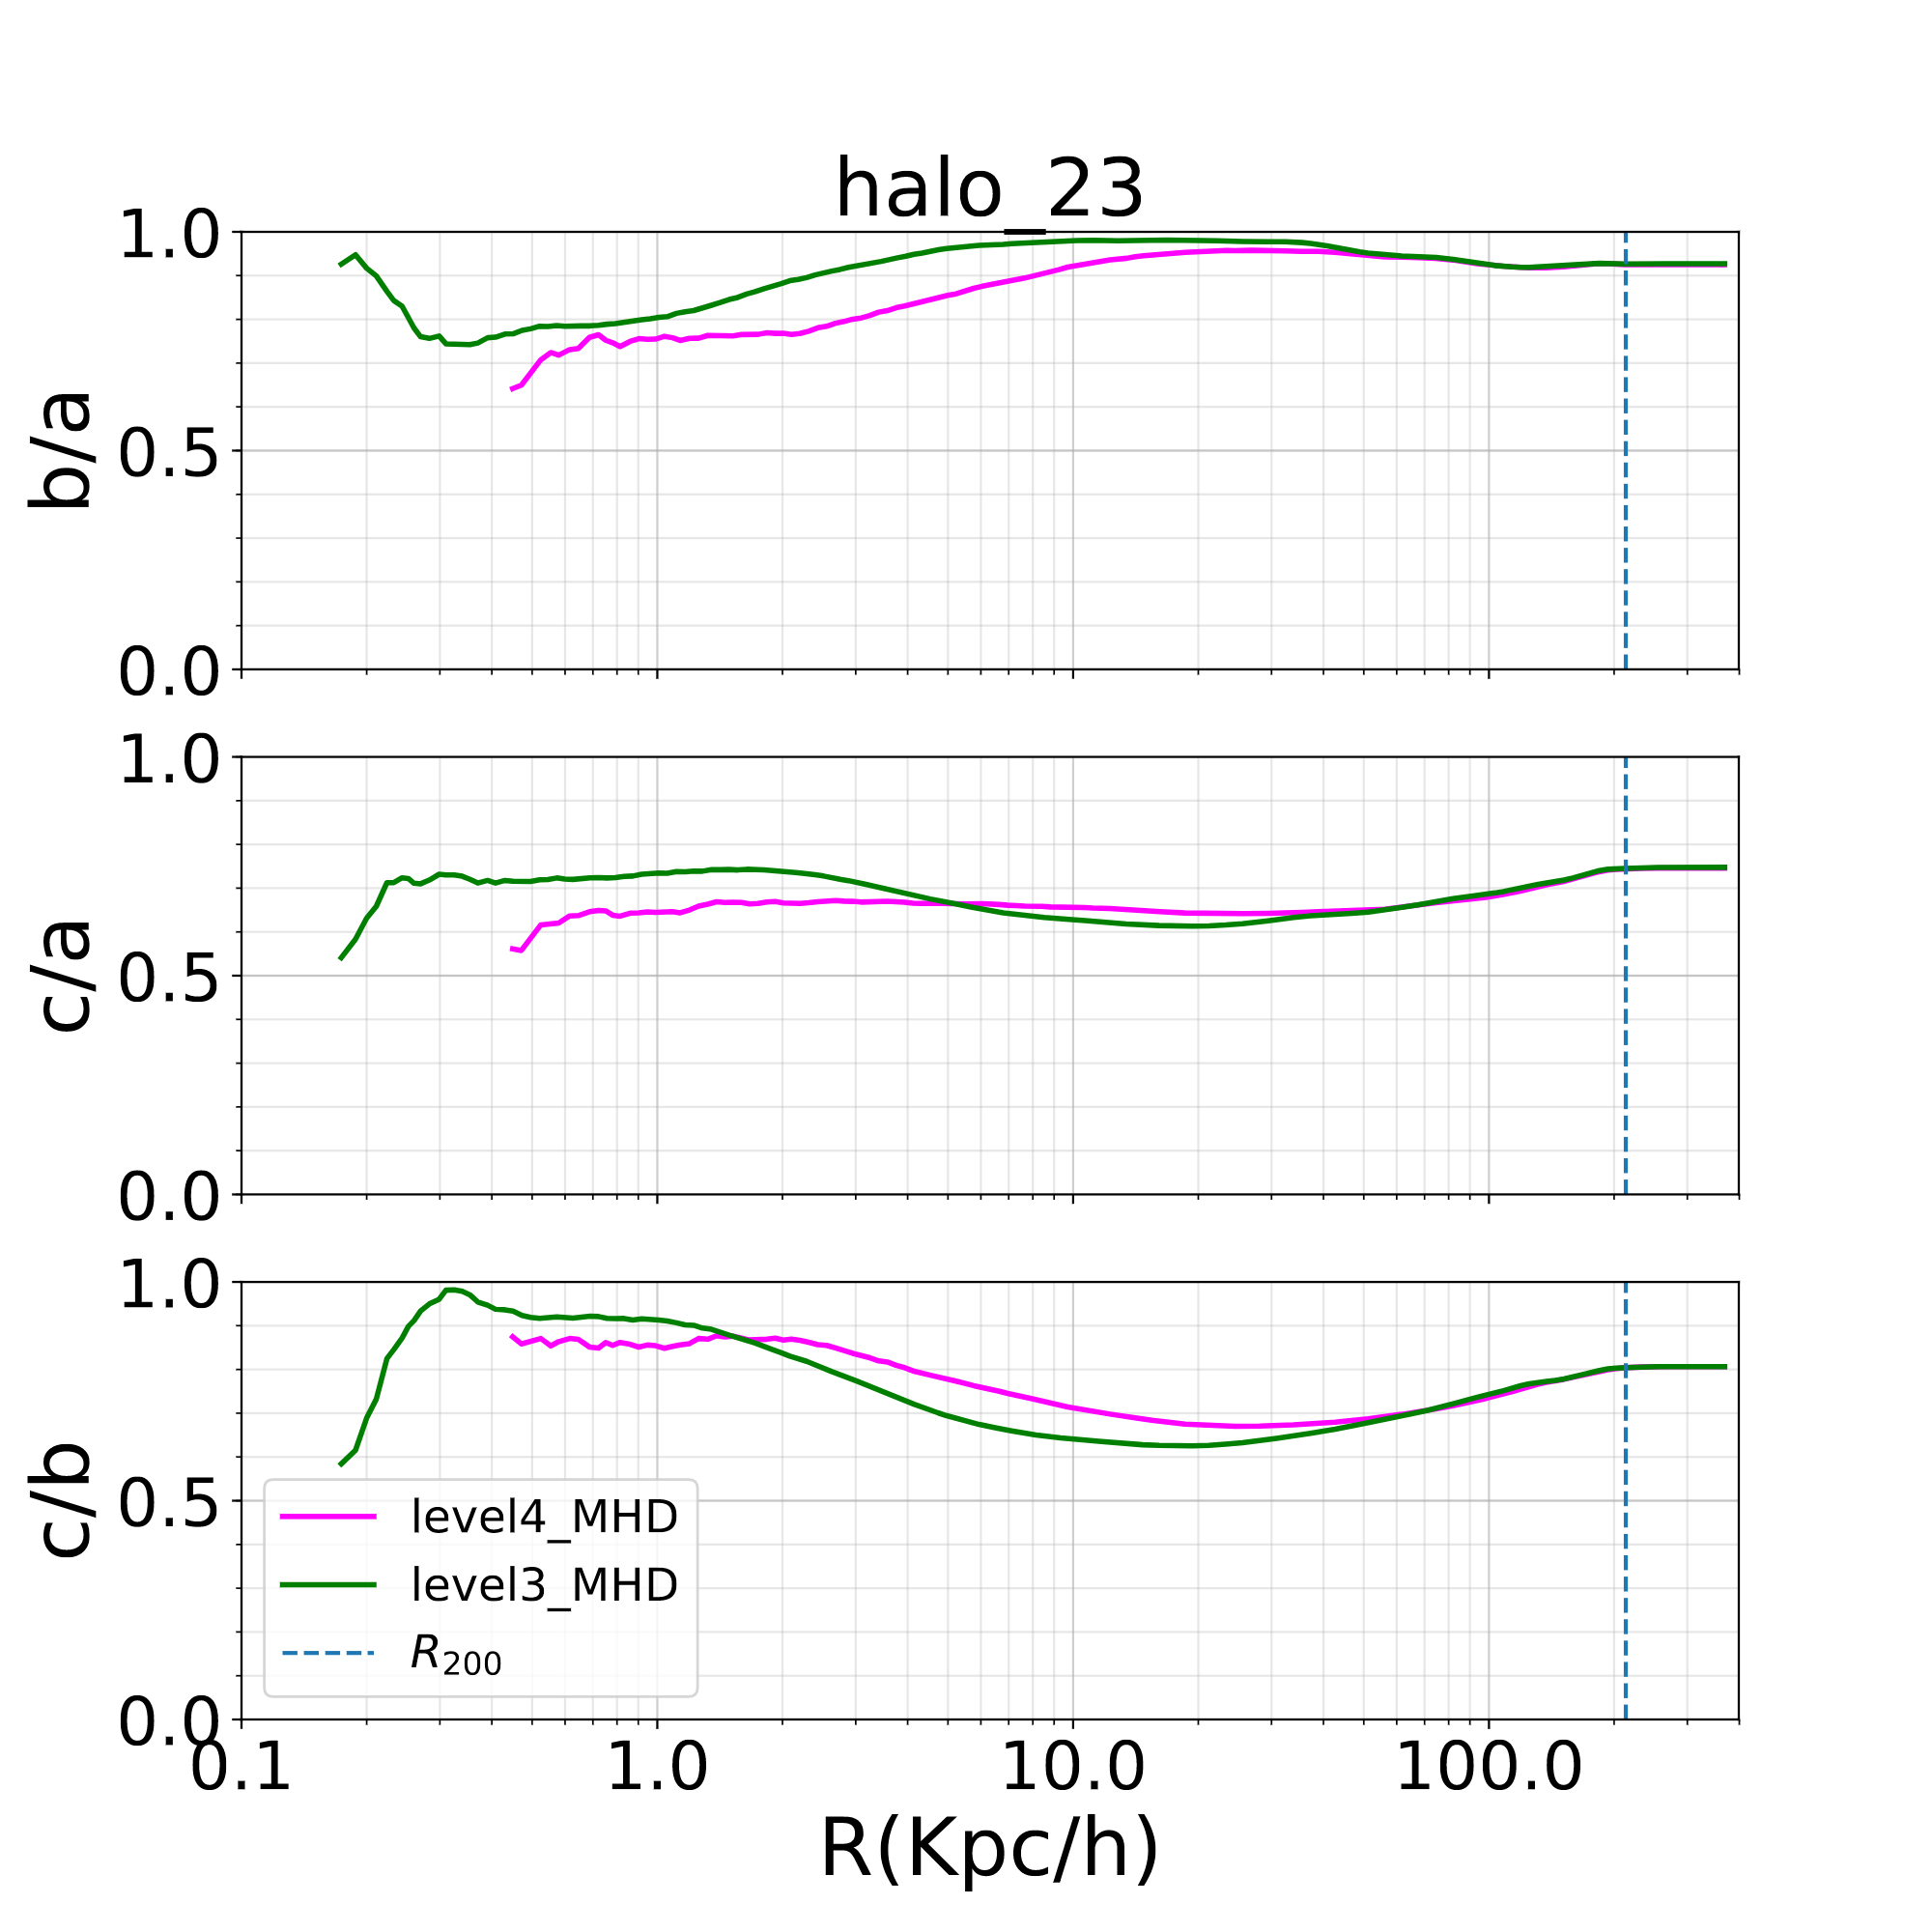
\includegraphics[width=0.5\columnwidth]{./pics/Convergence/halo23_MHD_3Vs4_bad.png}\label{fig:badConvergenceMHD}}
  \caption{Examples of halos where resolution had an appreciable effect on the halo shape. There is an appreciable difference between level 3 (blue) and level 4 (red) calculations. However it does not modify the halo's shape in any specific way. \textbf{put labels, bigger axes font, add title} }
\end{figure}


We decided to analyze de radial profiles at redshift 0 and compare level5 to level3 simulations. In general, the DM halo shapes remain unchanged with the exeption of the radial regimes where resolution becomes important. However, for MHD simulations, the resolution of gas affects the measurement not only in the inner parts, where resolution issues are evident, but it has a more global effect, presumably because of the scattering of particles which is also supporting the claim that matter affects the halo shape through scattering.\\

We address this problem by performing random sampling of the level3 simulations to reproduce level4 measurements and estimate the associated error.\\

\begin{figure}[!ht]
  \centering
  \subfloat[halo 24 MHD]{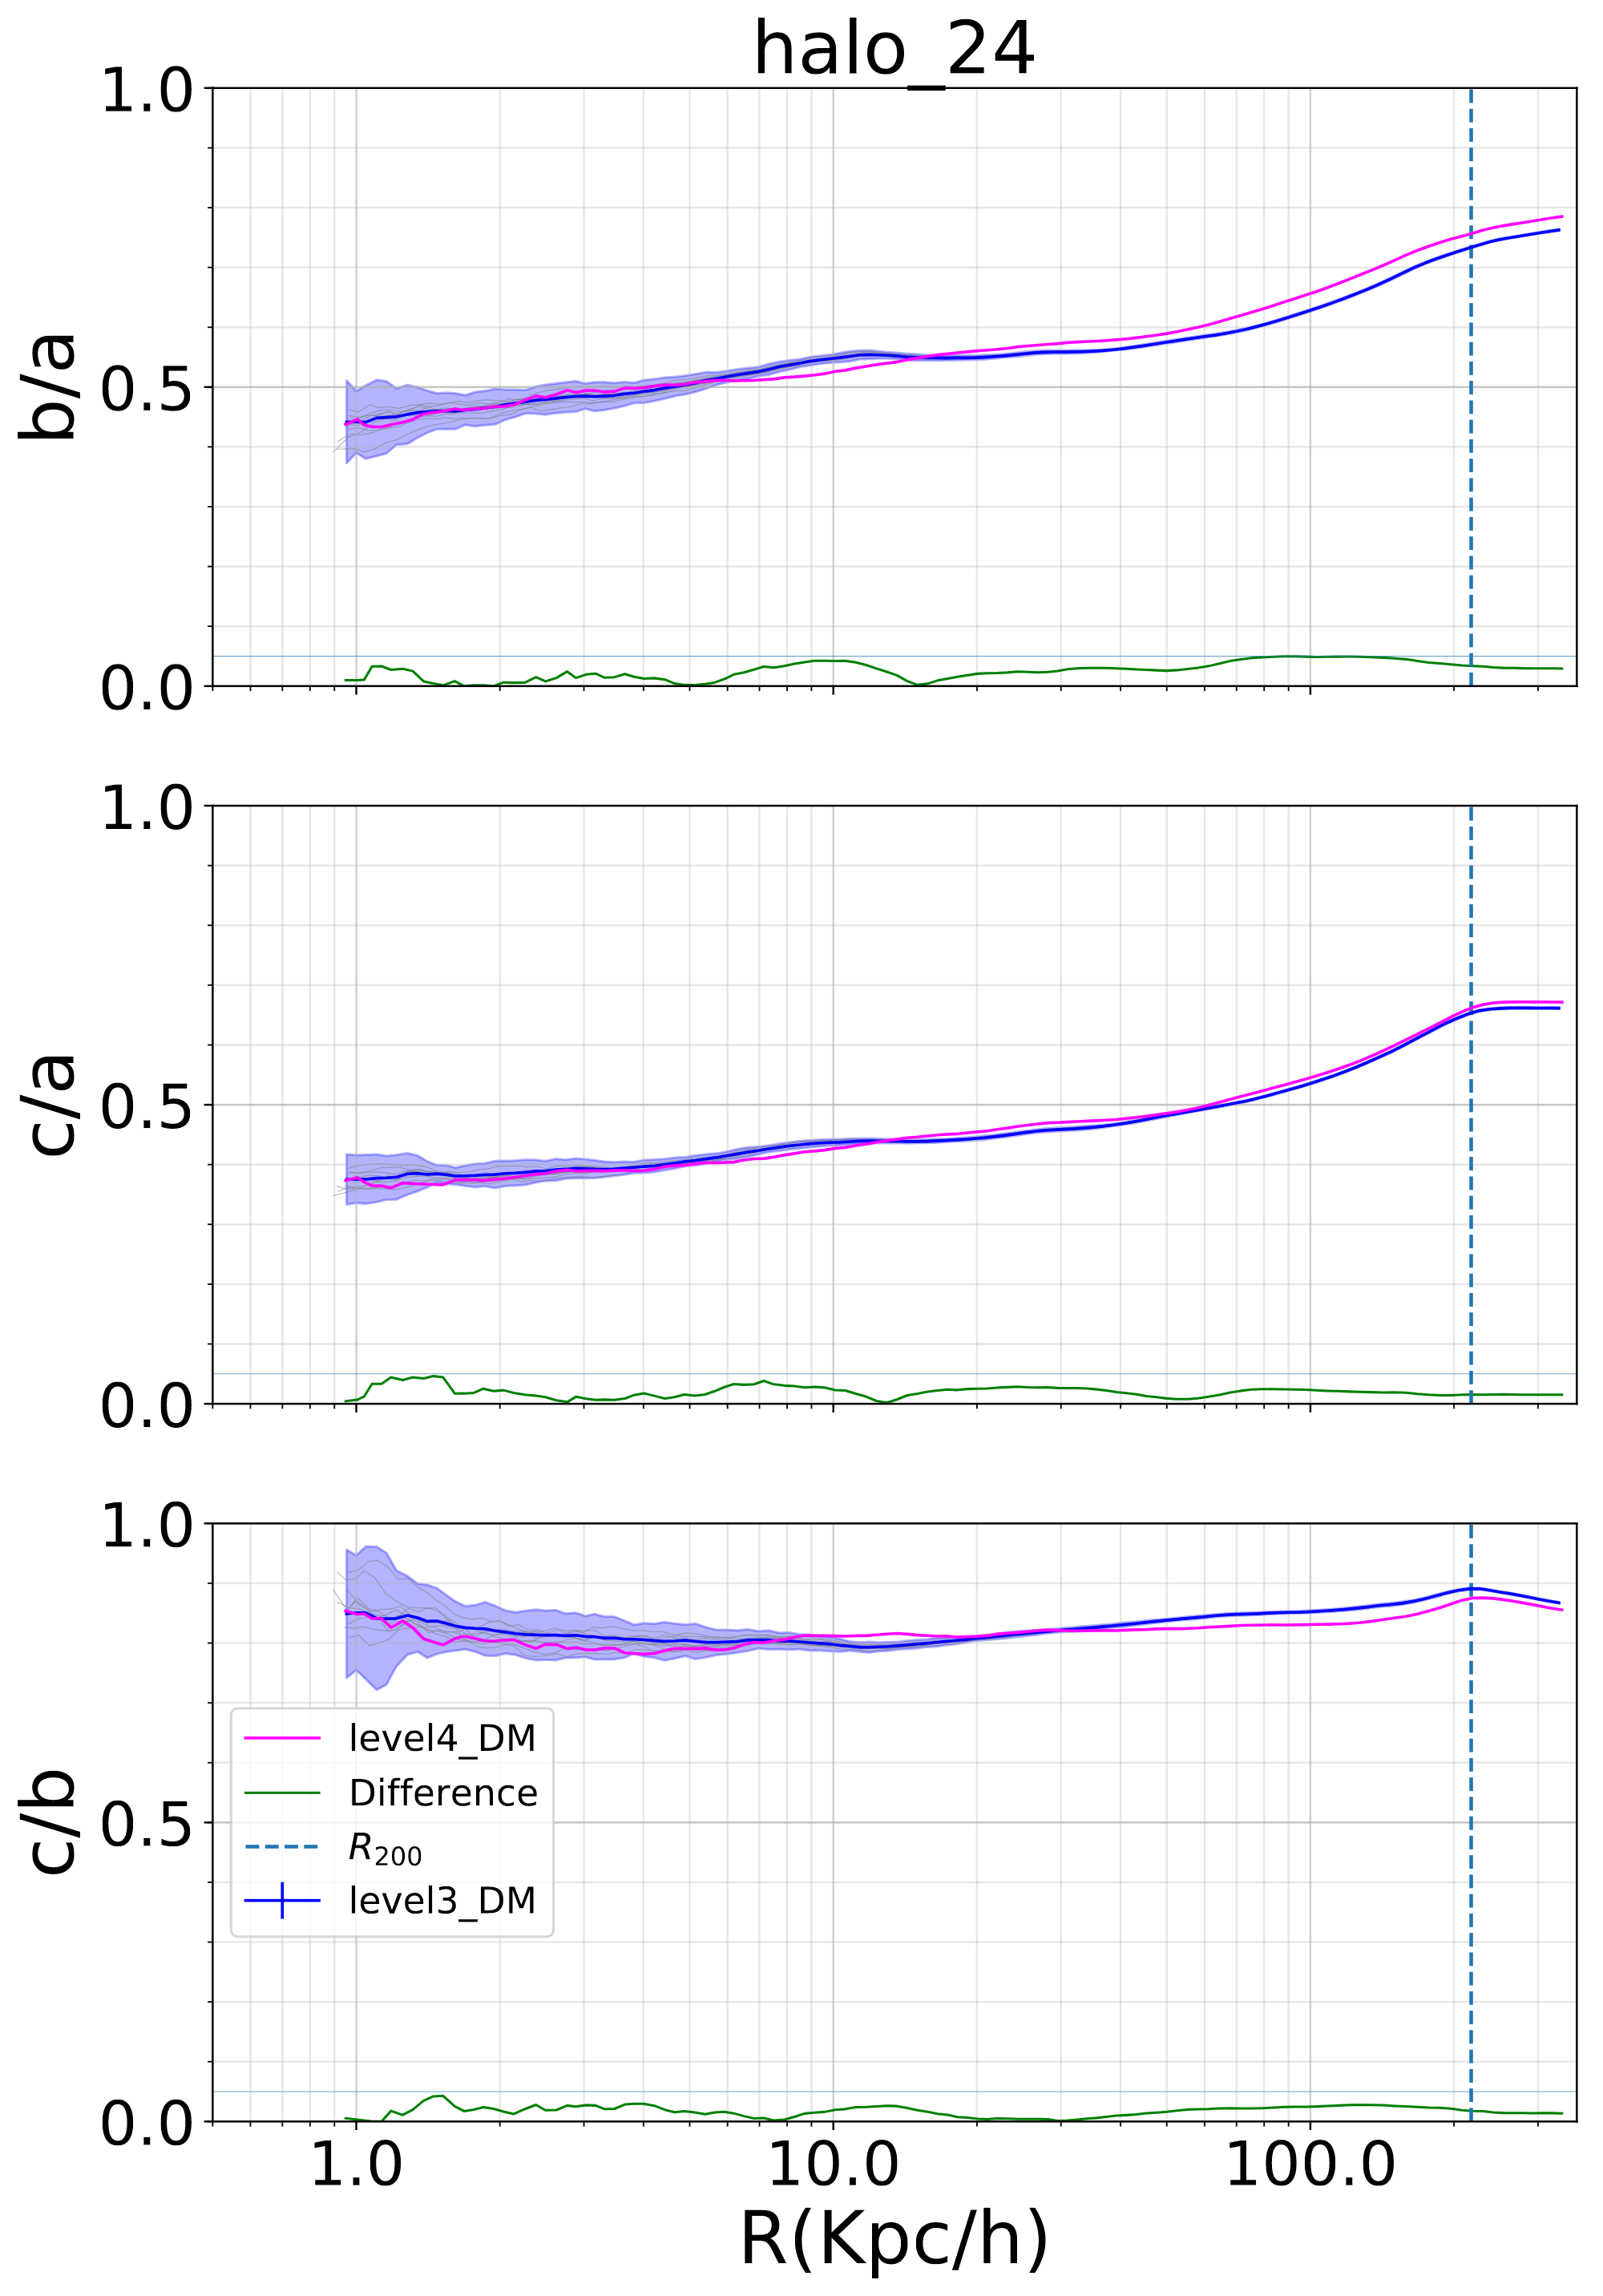
\includegraphics[width=0.5\columnwidth]{./pics/Convergence/rand_conv_halo24_DM.png}\label{fig:convergenceMHD}}
  \hfill
  \subfloat[halo 24 DM]{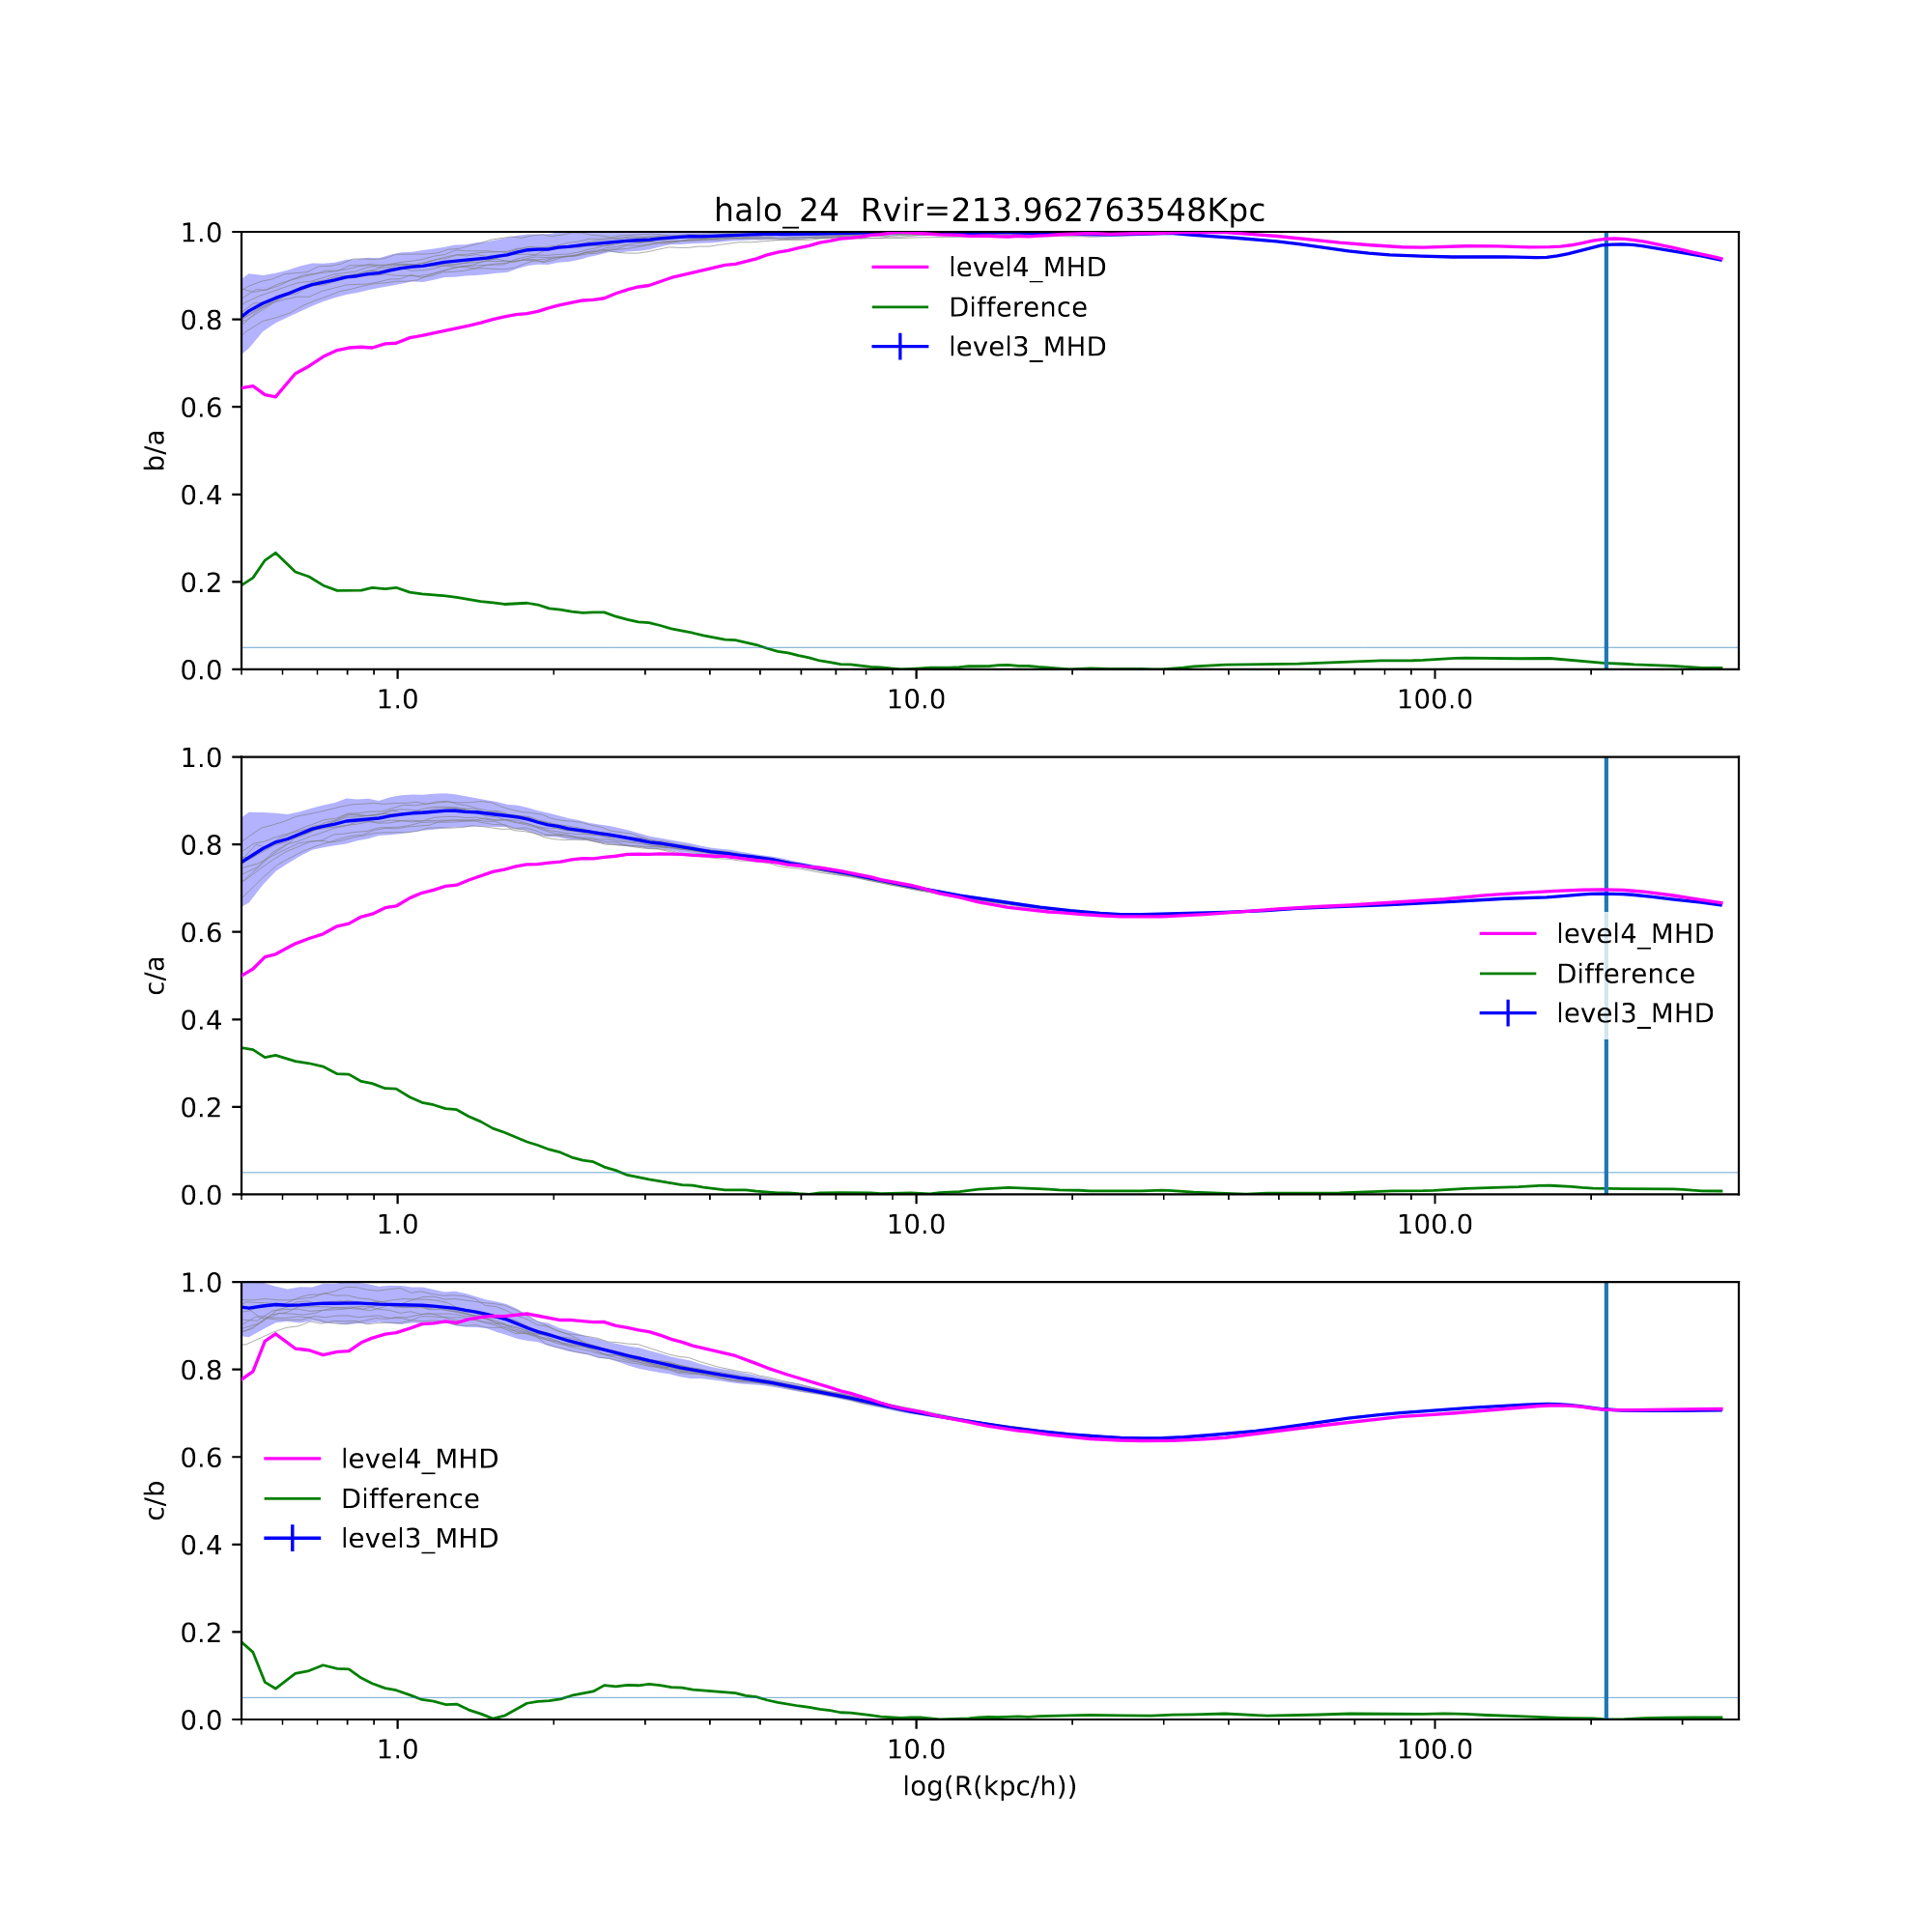
\includegraphics[width=0.5\columnwidth]{./pics/Convergence/rand_conv_halo24_MHD.png}\label{fig:convergenceDM}}
  \caption{Comparison of the effect of resolution on DM and MHD simualations. Here level4 curves (magenta) are compared to the mean and 2std (confirm) of the random-sampled curves from level3. For better comparison of the effect of resolution, the difference percent is plotted in green.  \textbf{bigger axes font}}
\end{figure}



State the main conclusions about this analysis of convergence. The effect of particle resolution does not sistematically affect the measurements. However, the error produced is specially apreciable at inner parts where for MHD it has a more global effect through scattering.\\

Halo shape is heavily determined by accretion with environment \cite{shape relation with environment}. As environment may also be affected by resolution, this may have an effect on the halo shape. Also, resolution discrepancies may snowball through history.

\section{The shape's radial dependence}
One of the first results we obtained in this work is related to the impact of the radius on the shape. Halos accrete mass from inner shells to outter shells. Inner shells are isolated from outter regions (gauss law effect?) and tend to conserve their shape (angular momentum?). Outter shells, on the other side are affected by the inner gravitational potential and is prone to scattering effects. This has a "rounding" effect on the halo shape. For this reason, we expect on both simulations (lvl3MHD,lvl3DM) that halos are more triaxial on inner regions and more spherical at bigger radii.\\


\begin{figure}[!ht]
  \centering
  \subfloat[halo 27 DM shape at small radius]{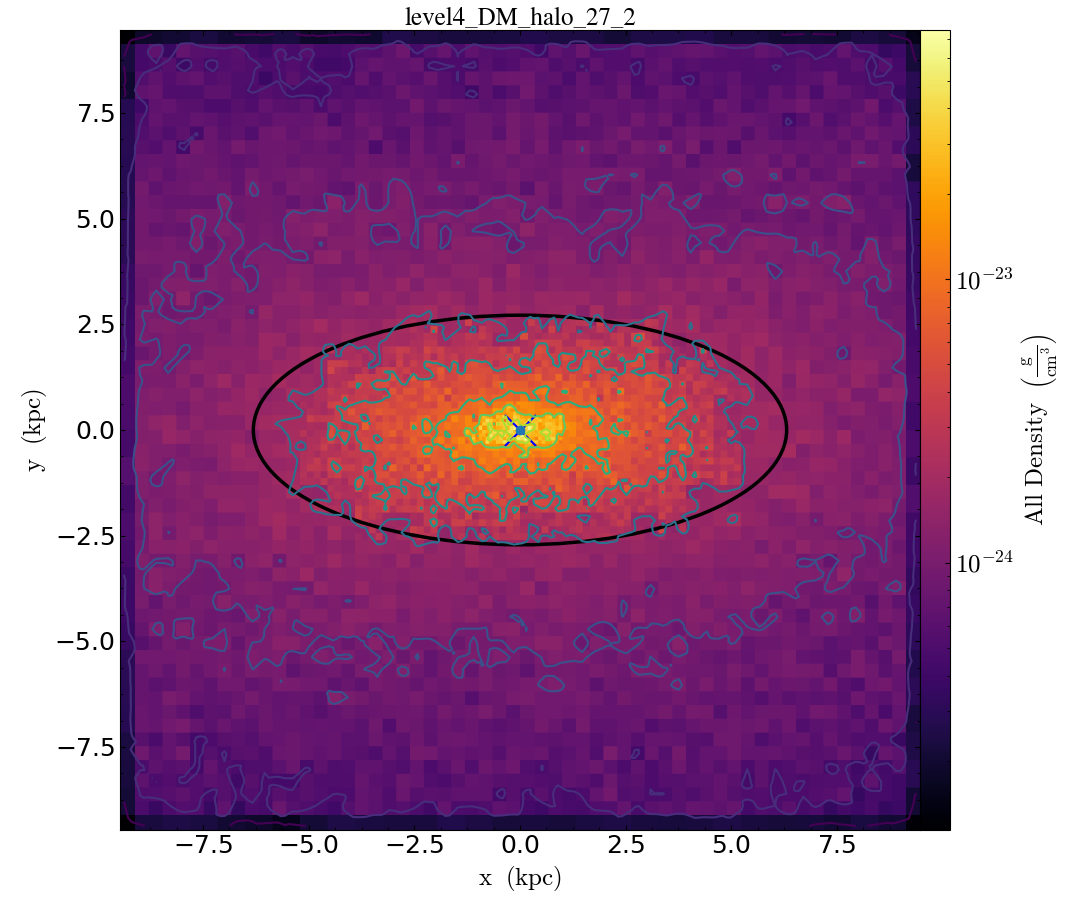
\includegraphics[width=0.5\columnwidth]{./pics/MHD_Vs_DM/level4_DM_halo_27_inner.png}\label{fig:innerDM}}
  \hfill
  \subfloat[halo 27 DM shape at big radius]{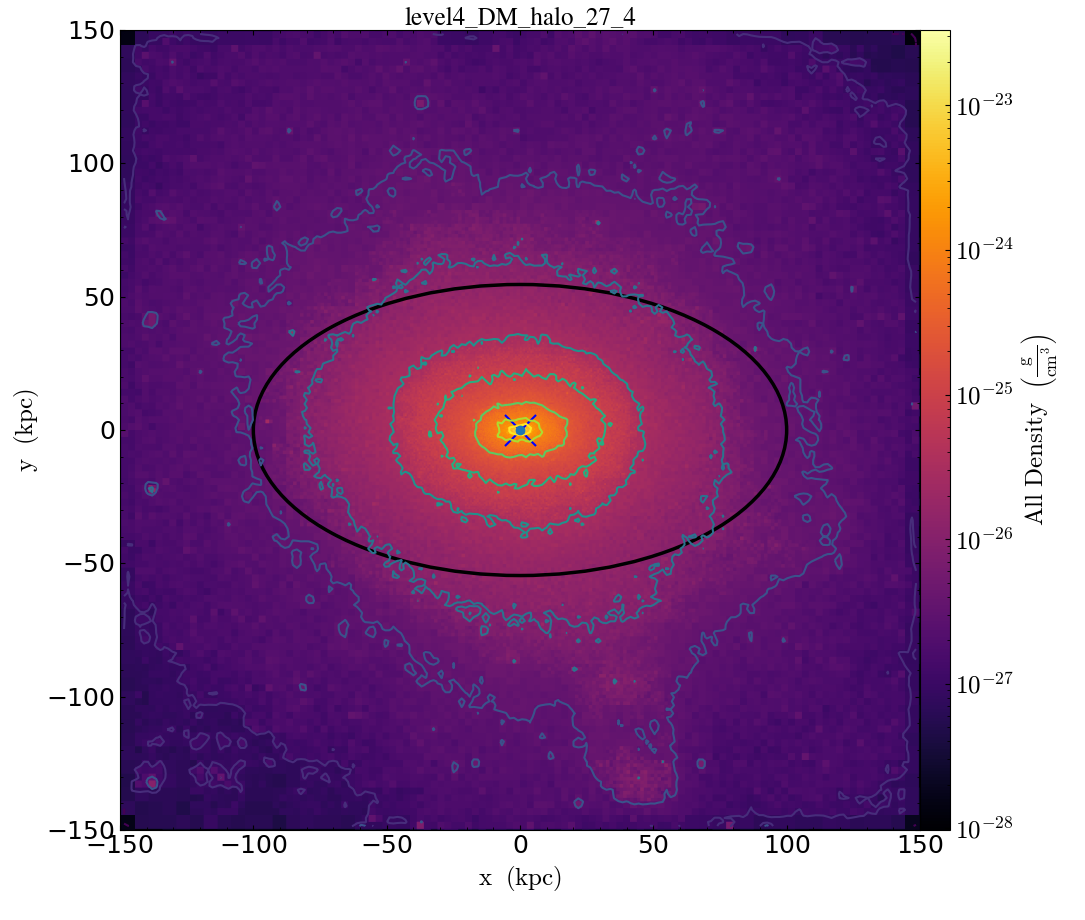
\includegraphics[width=0.5\columnwidth]{./pics/MHD_Vs_DM/level4_DM_halo_27_outter.png}\label{fig:outterDM}}
  \hfill
  \subfloat[halo 27 MHD shape at small radius]{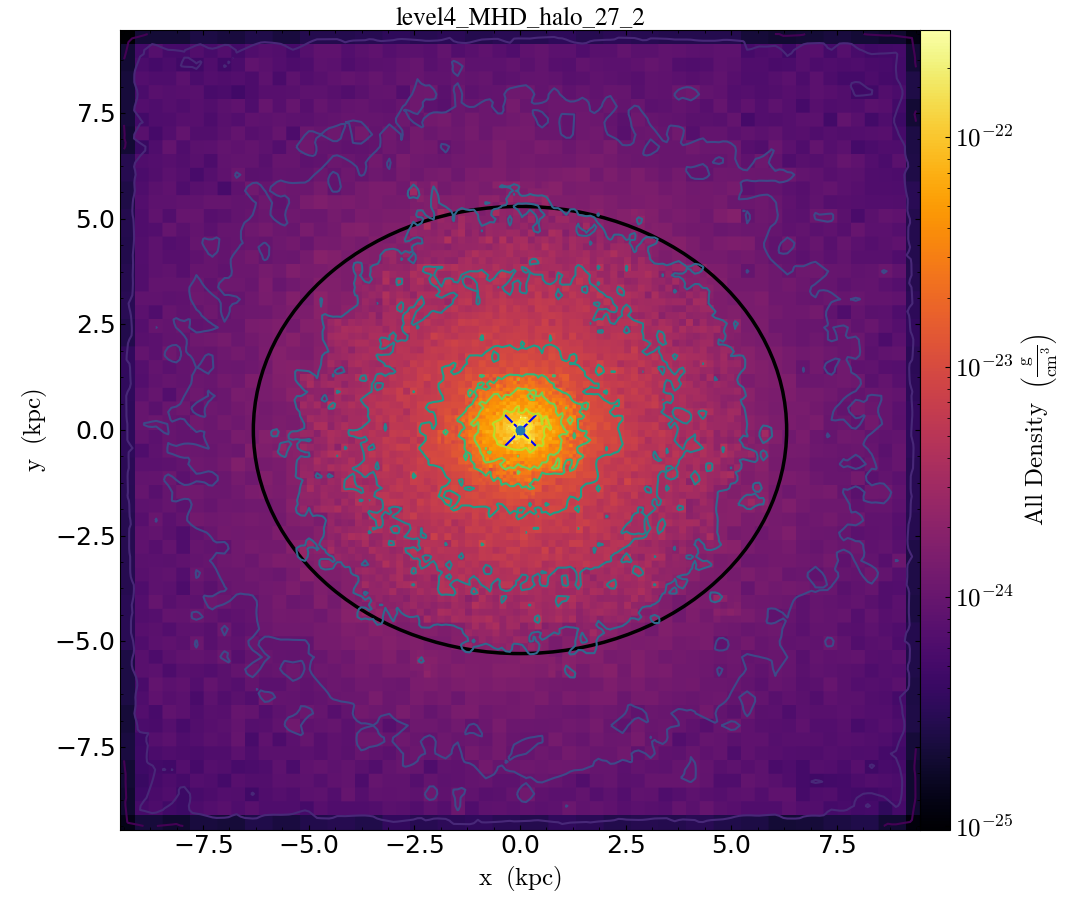
\includegraphics[width=0.5\columnwidth]{./pics/MHD_Vs_DM/level4_MHD_halo_27_inner.png}\label{fig:innerMHD}}
  \hfill
  \subfloat[halo 27 MHD shape at big radius]{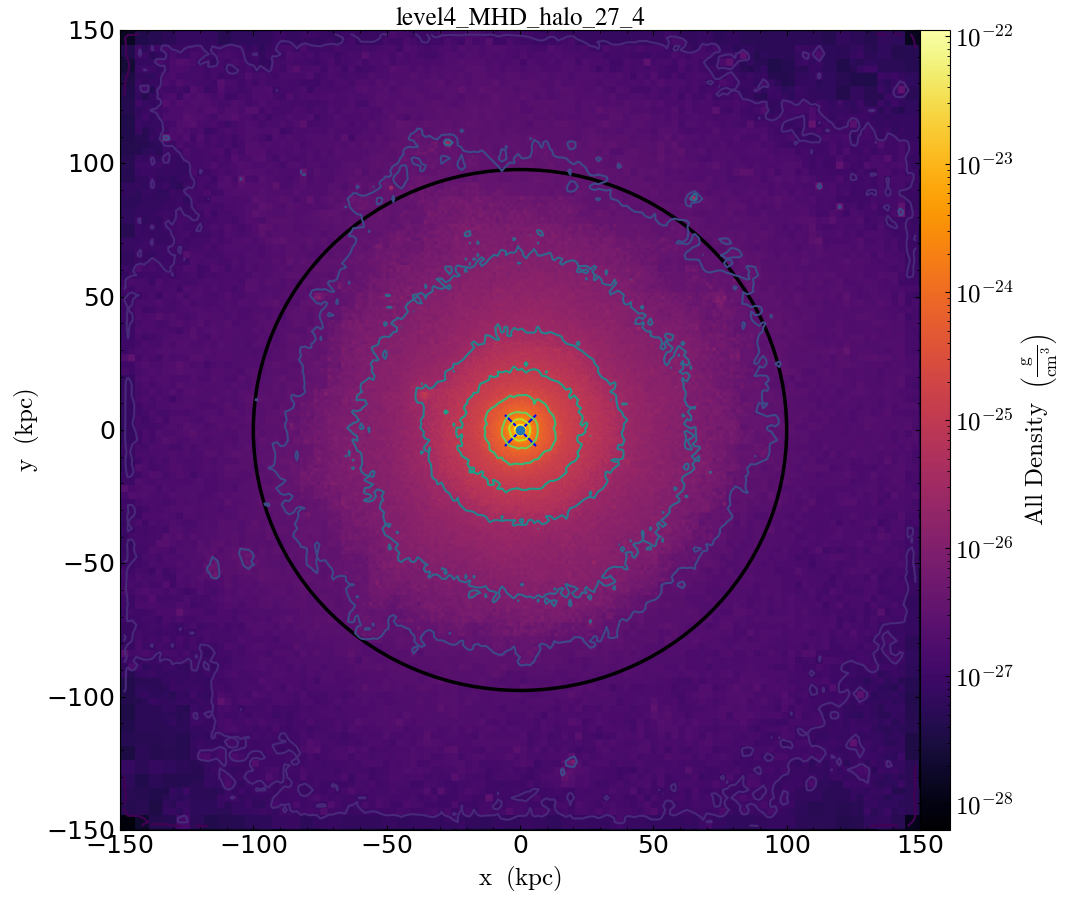
\includegraphics[width=0.5\columnwidth]{./pics/MHD_Vs_DM/level4_MHD_halo_27_outter.png}\label{fig:outterMHD}}
  \caption{Example of the dependence of shape in terms of the radius. All graphics have matching orientation (which may not be the same) with their respective principal axes at the shown radii. The horizontal and vertical axes correspond to the major and medium semi-axes respectively. }
\end{figure}

\subsection{The effect of gas on the halo shape}
The rounding effect with radius is specially evident in this example, but it is a general tendency over all. From this comparison we can notice that there is also a relation of this roundong effect with the presence of matter, which is to be expected. Unlike DM, gas collapses and generate disks which are much denser than DM at the scales where it forms. This amplifies scattering events and if we apply the same logic, we would expect that the inner regions of the halo are more spherical when there is presence of DM. We expect the same for outter regions but this effect is expected to be more significant due to the stronger effect of the gravitational potential on the outter shells.\\

\begin{figure}
\centering
{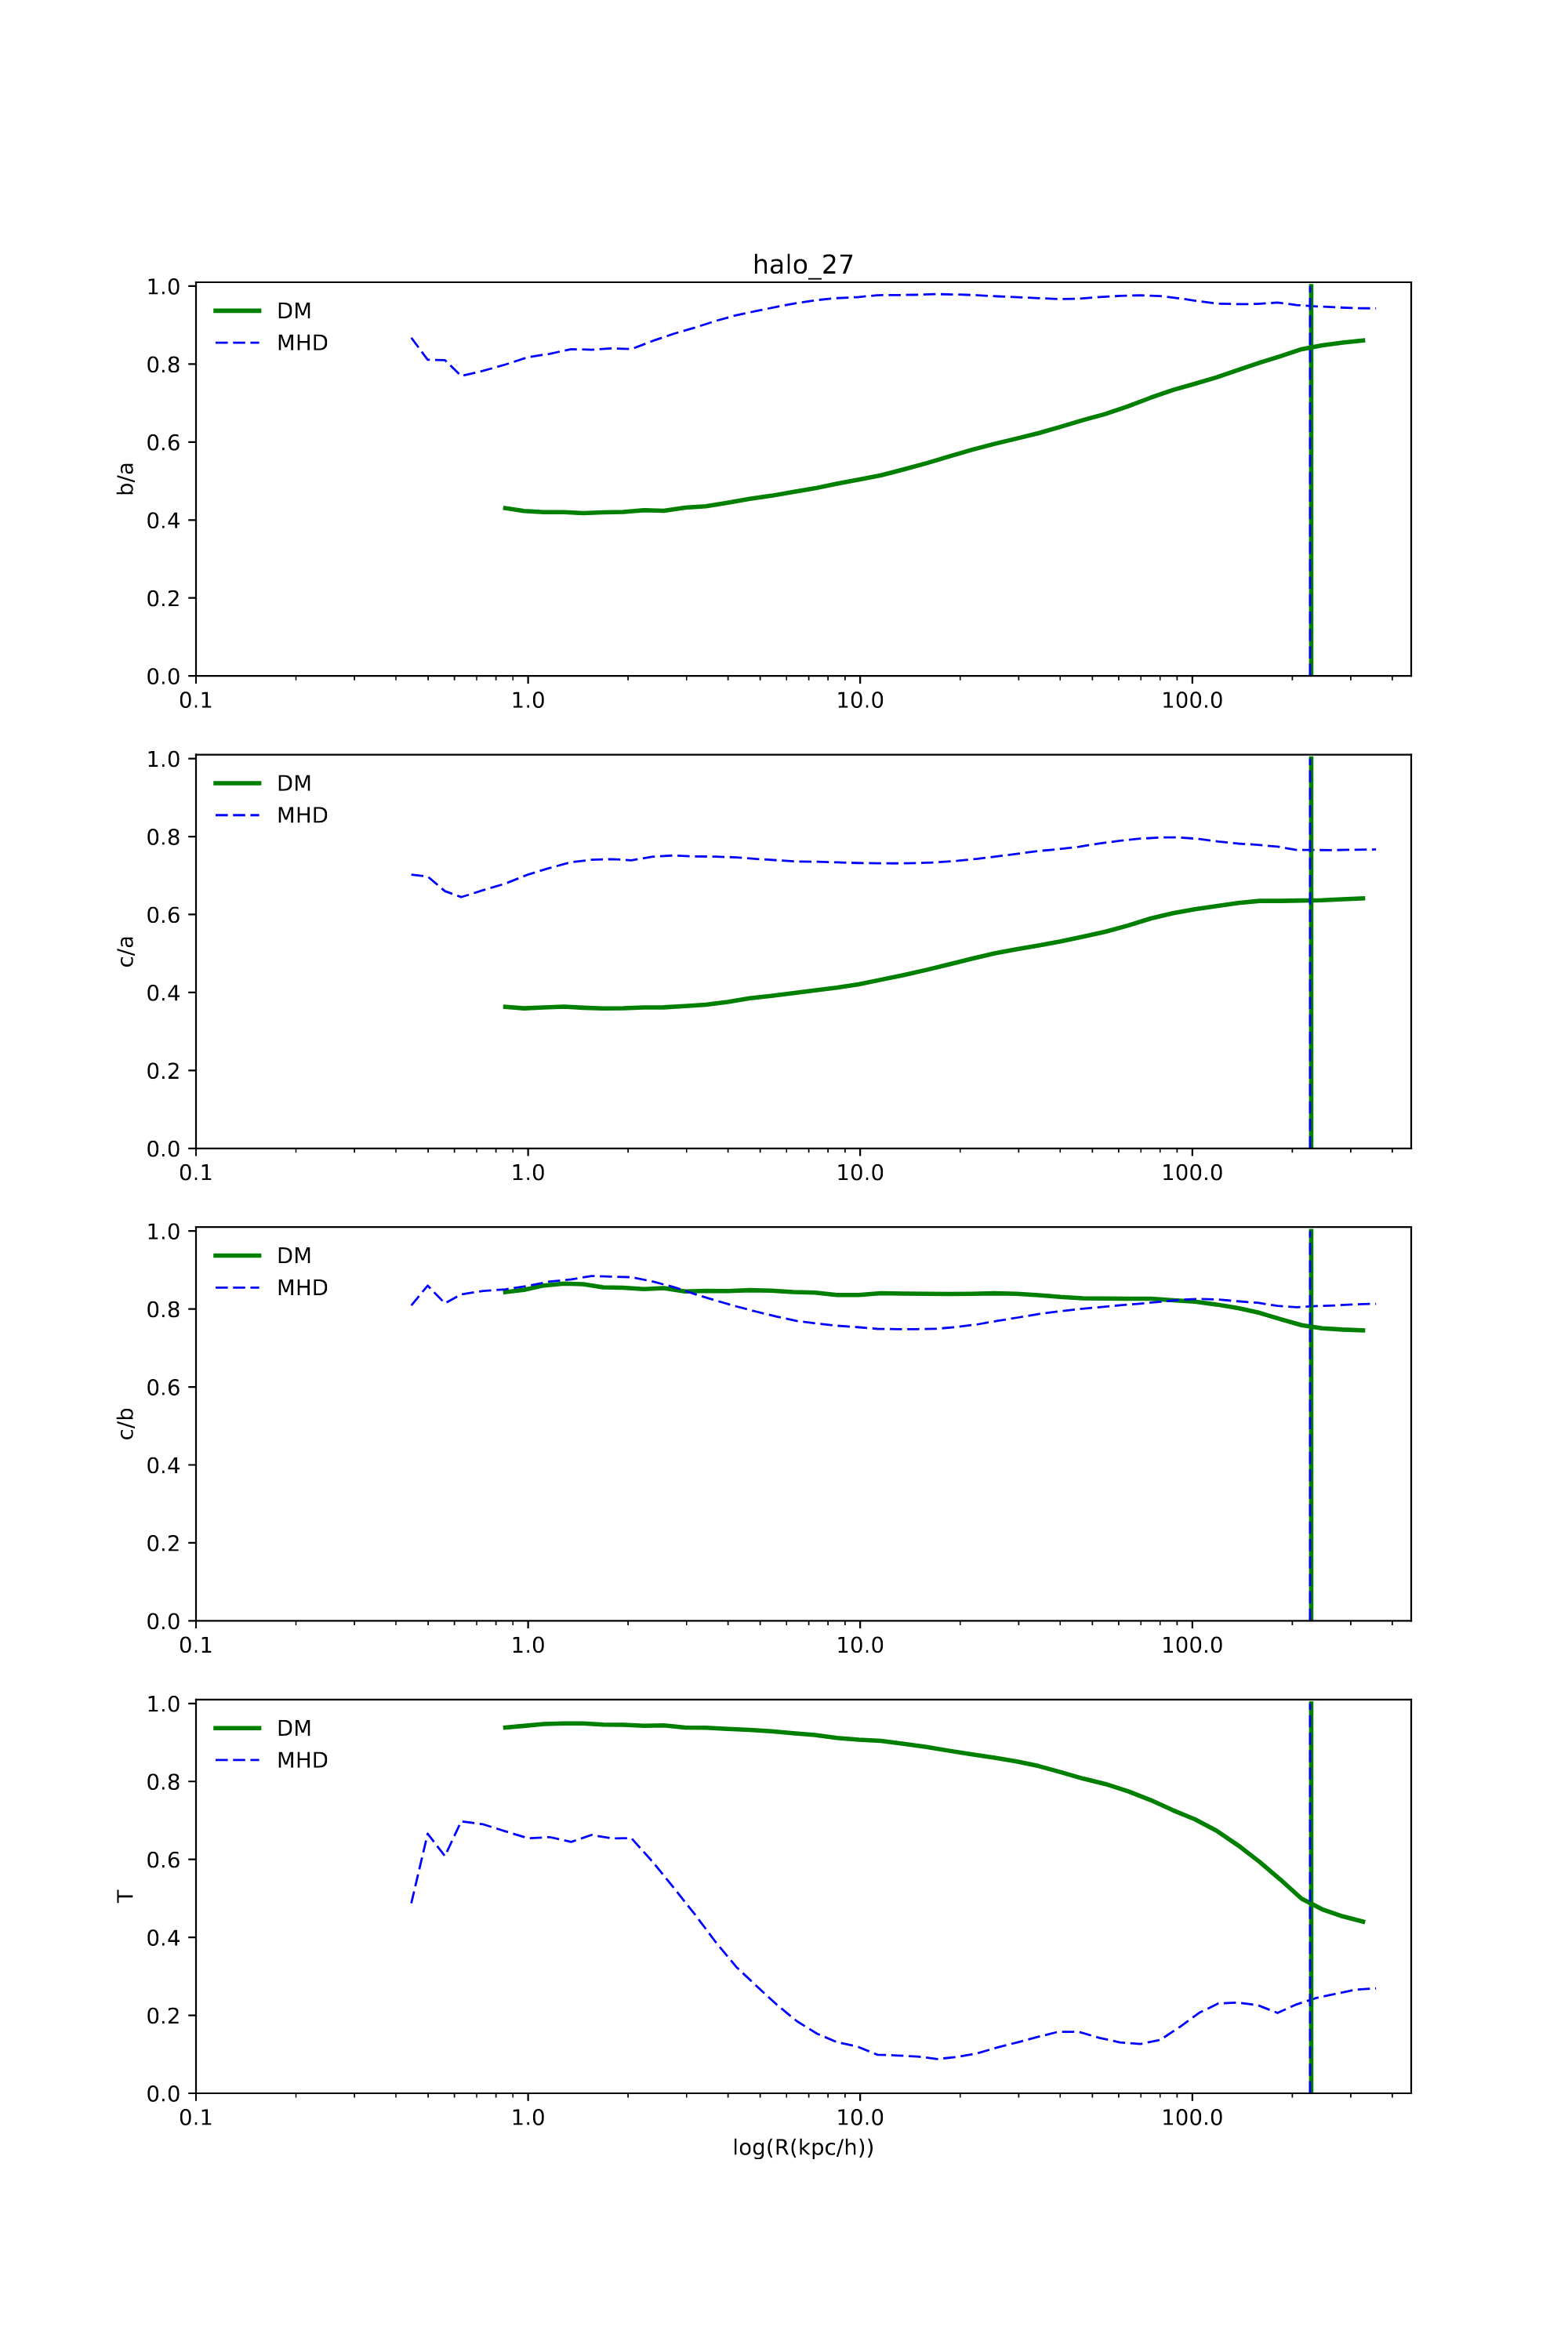
\includegraphics[width=1\columnwidth]{./pics/MHD_Vs_DM/level4_halo_27_DM_Vs_MHD.png}\label{fig:outterMHD}}
\caption{Semi-axial ratios and triaxiality $\frac{1-b/a}{1-c/a}$ as function of radius for semi-axes $a\geq b\geq c$. The MHD simulation (blue dotted line) shows ratios closer to $1$ than those from the DM-only (green solid line) simulation. The rounding effect with radius for each simulation separatedly is also well-appreciable in this graphic. The radial-rounding, as well as the gas-presence amplification can be evidenced on the triaxiality function. \textbf{show two examples or reorganize subplots to get a square figure, bigger label and axes font}}
\end{figure} 

The general tendency can be better visualized on the triaxial plane (explain what is that).

\begin{figure}[!ht]
  \centering
  \subfloat[Level3 MHD Vs DM at inner regions]{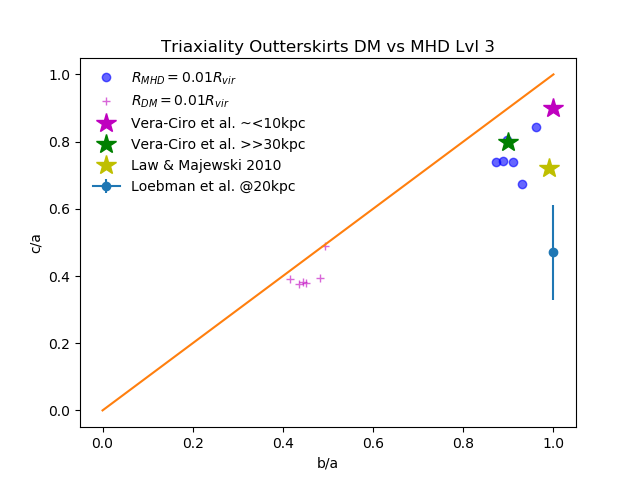
\includegraphics[width=0.5\columnwidth]{./pics/Triaxial_Plane/Triaxiality_Inner_lvl3.png}\label{fig:innerTriaxial3}}
  \hfill
  \subfloat[Level3 MHD Vs DM at outter regions]{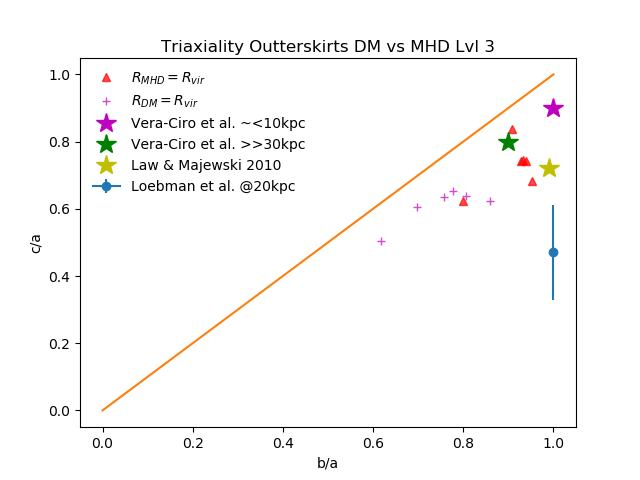
\includegraphics[width=0.5\columnwidth]{./pics/Triaxial_Plane/Triaxiality_Outer_lvl3.png}\label{fig:outterTriaxial3}}
  \hfill
  \centering
  \subfloat[Level4 MHD Vs DM at inner regions]{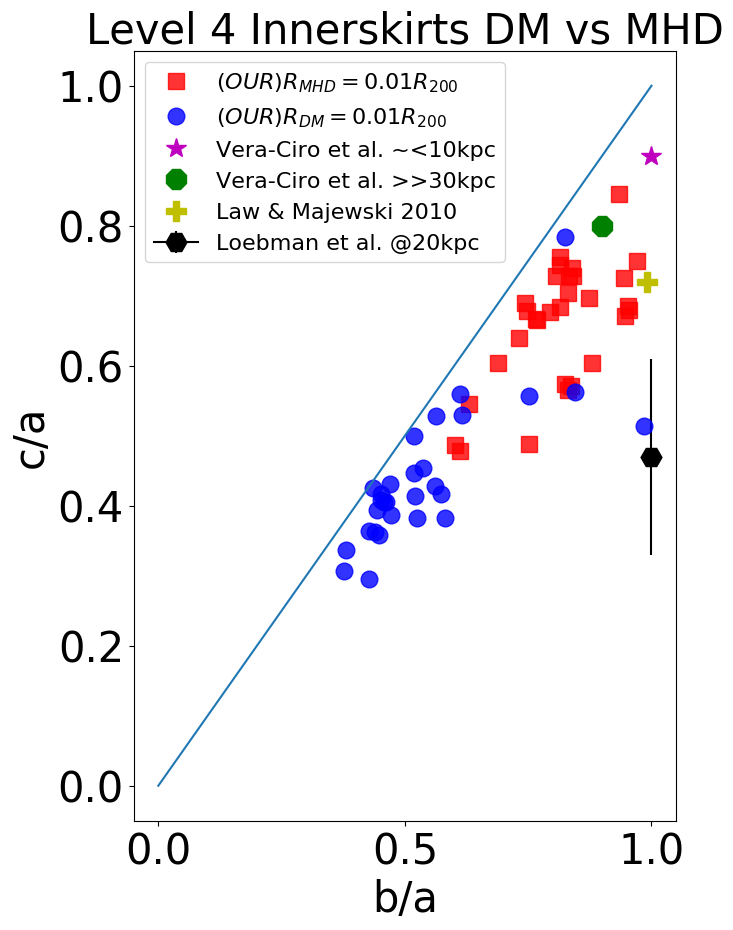
\includegraphics[width=0.5\columnwidth]{./pics/Triaxial_Plane/Triaxiality_Inner_lvl4.png}\label{fig:innerTriaxial4}}
  \hfill
  \subfloat[Level4 MHD Vs DM at outter regions]{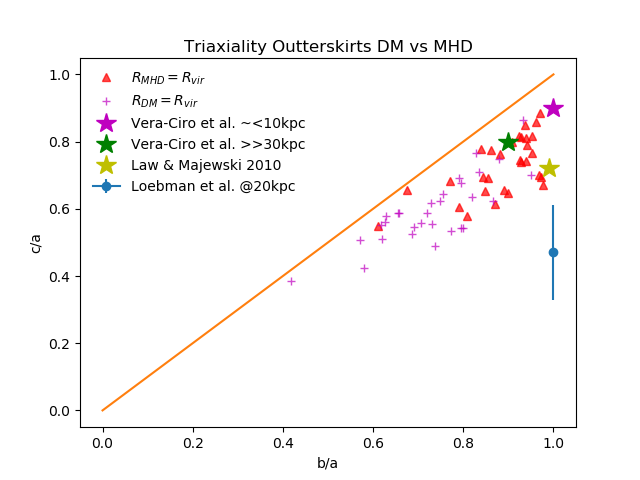
\includegraphics[width=0.5\columnwidth]{./pics/Triaxial_Plane/Triaxiality_Outer_lvl4.png}\label{fig:outterTriaxial4}}
  \hfill
  \caption{General tendence on the triaxial plane $c/a Vs b/a$. Some observational constraints (stars and error-bar point) are plotted alongside our results}
\end{figure}

\section{Historical shape}
Explain why it is expected for the shape to remain more or less constant with time: non-collisional DM, gauss law effect.


\begin{figure}[!ht]
  \centering
  \subfloat[halo 16 DM]{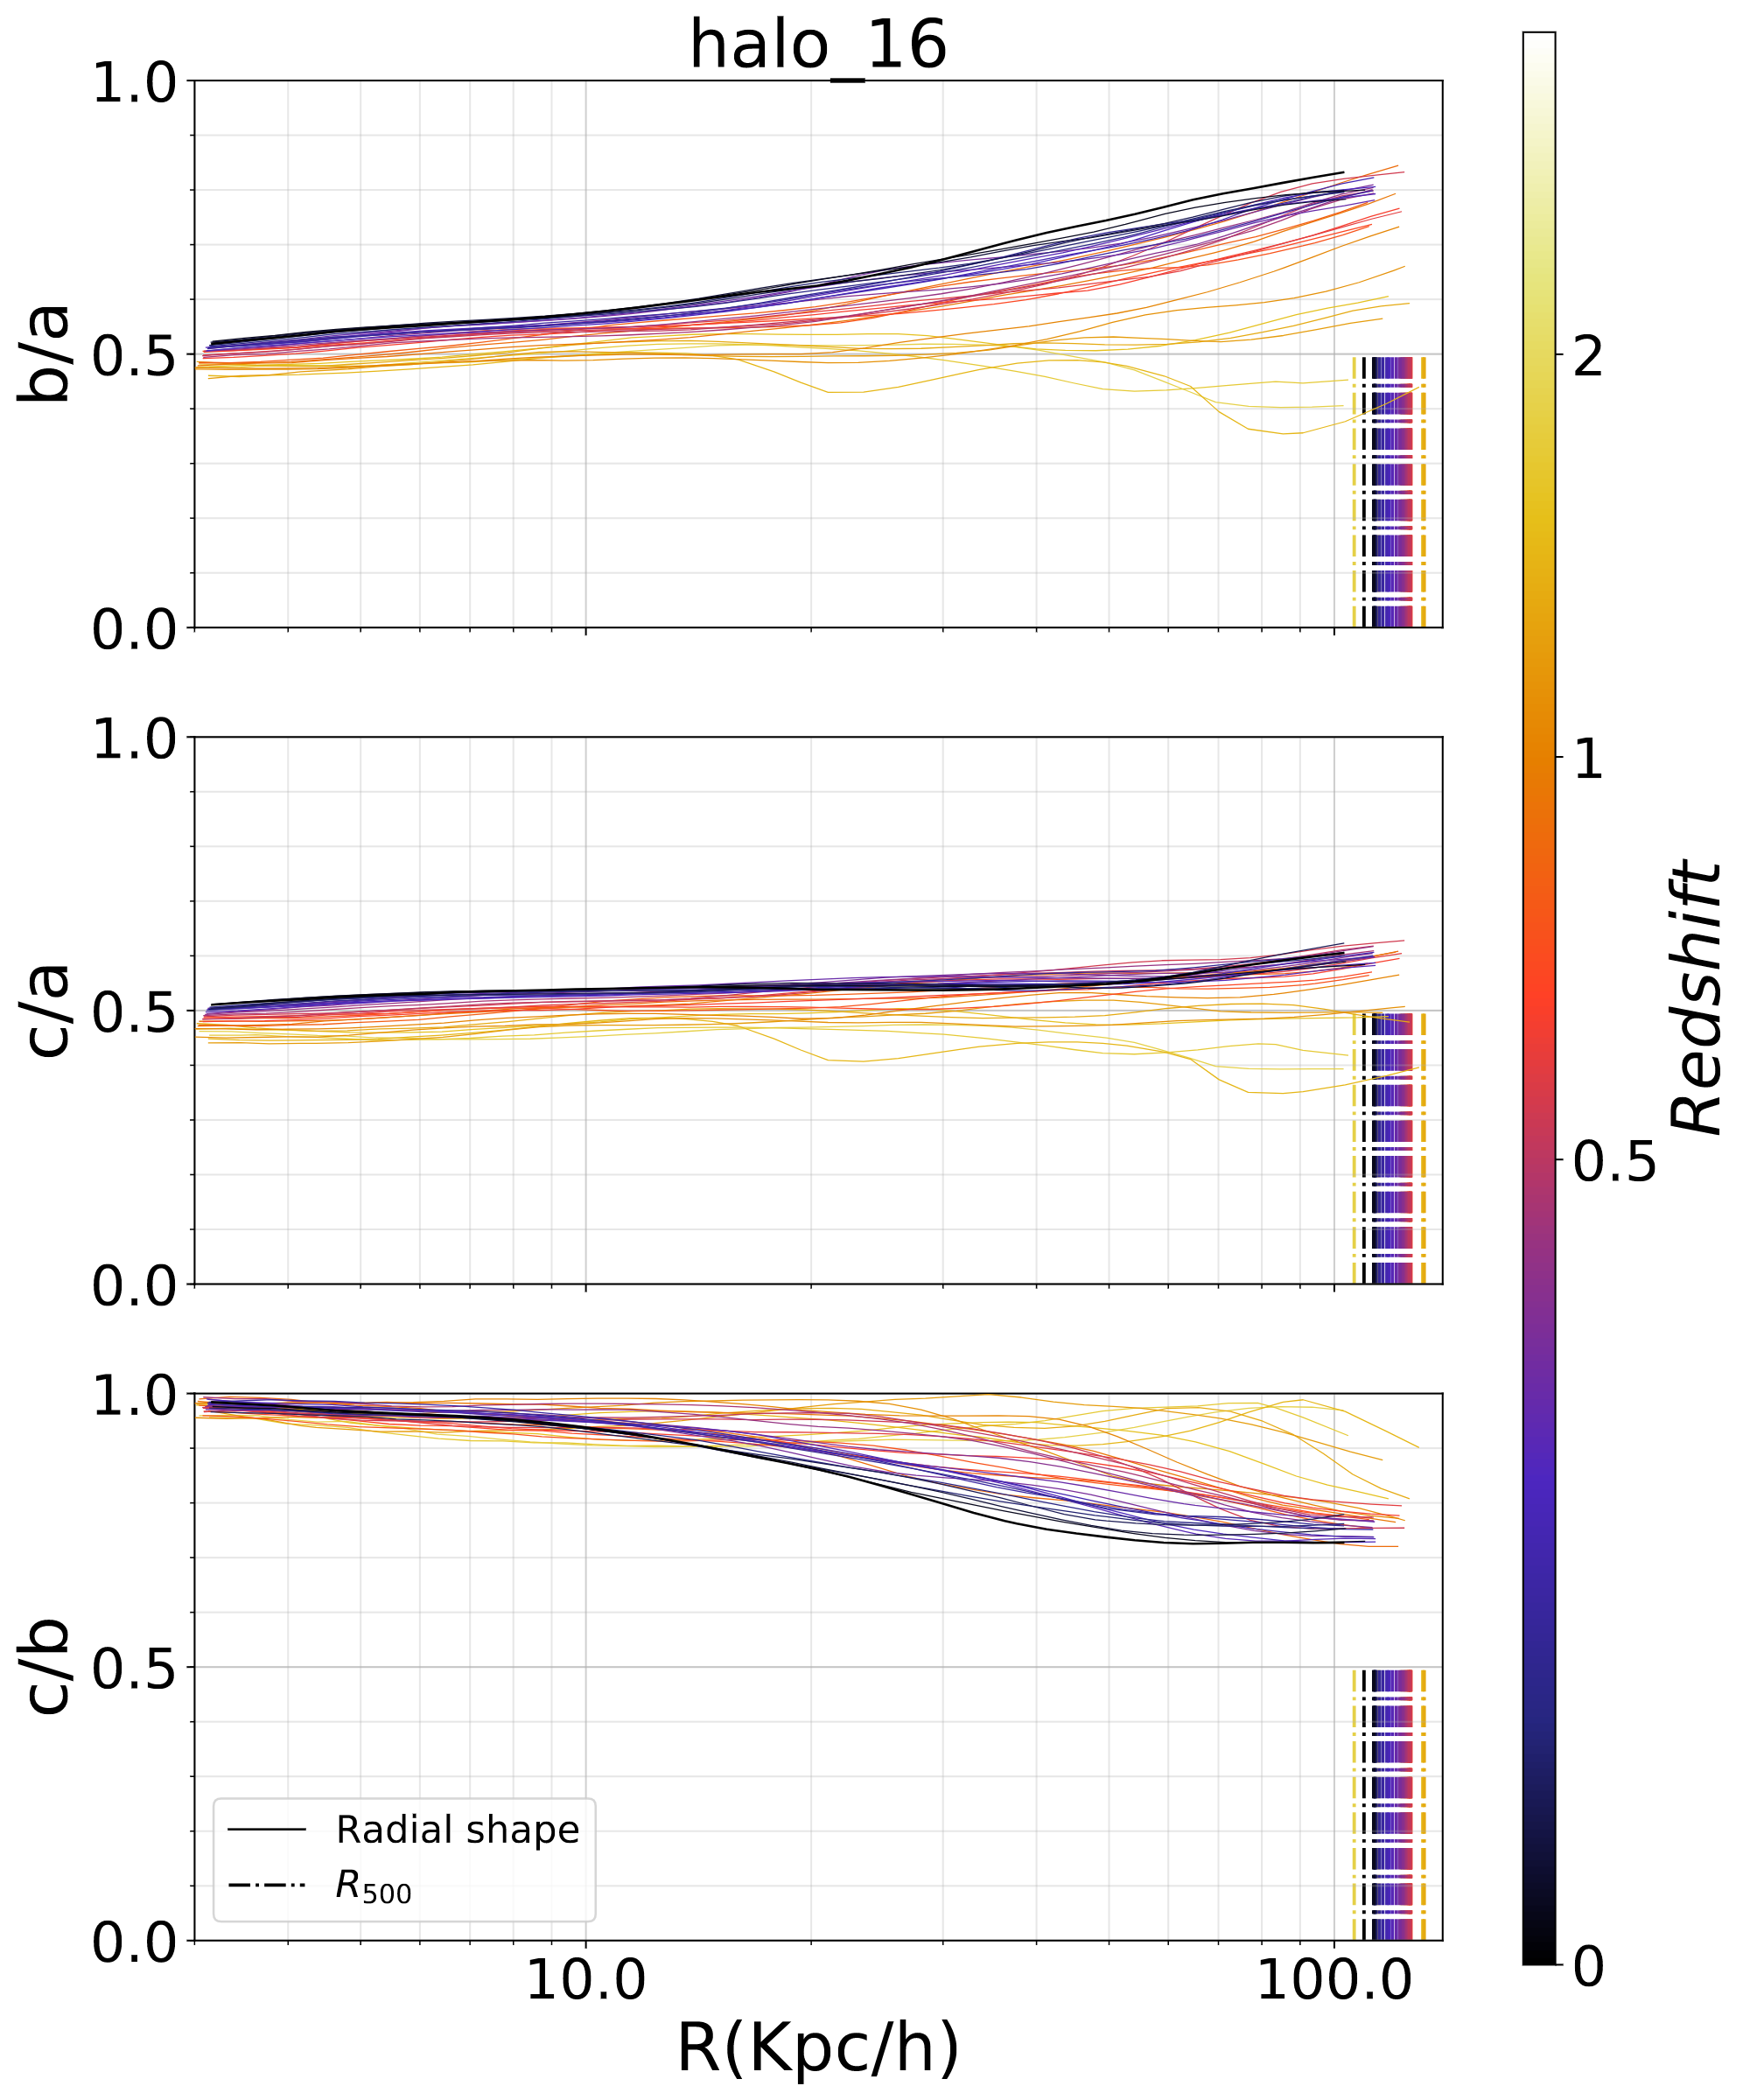
\includegraphics[width=0.5\columnwidth]{./pics/Redshift/halo_16_level3_DM_Z.png}\label{fig:RedshiftDMgood}}
  \hfill
  \subfloat[halo 16 MHD]{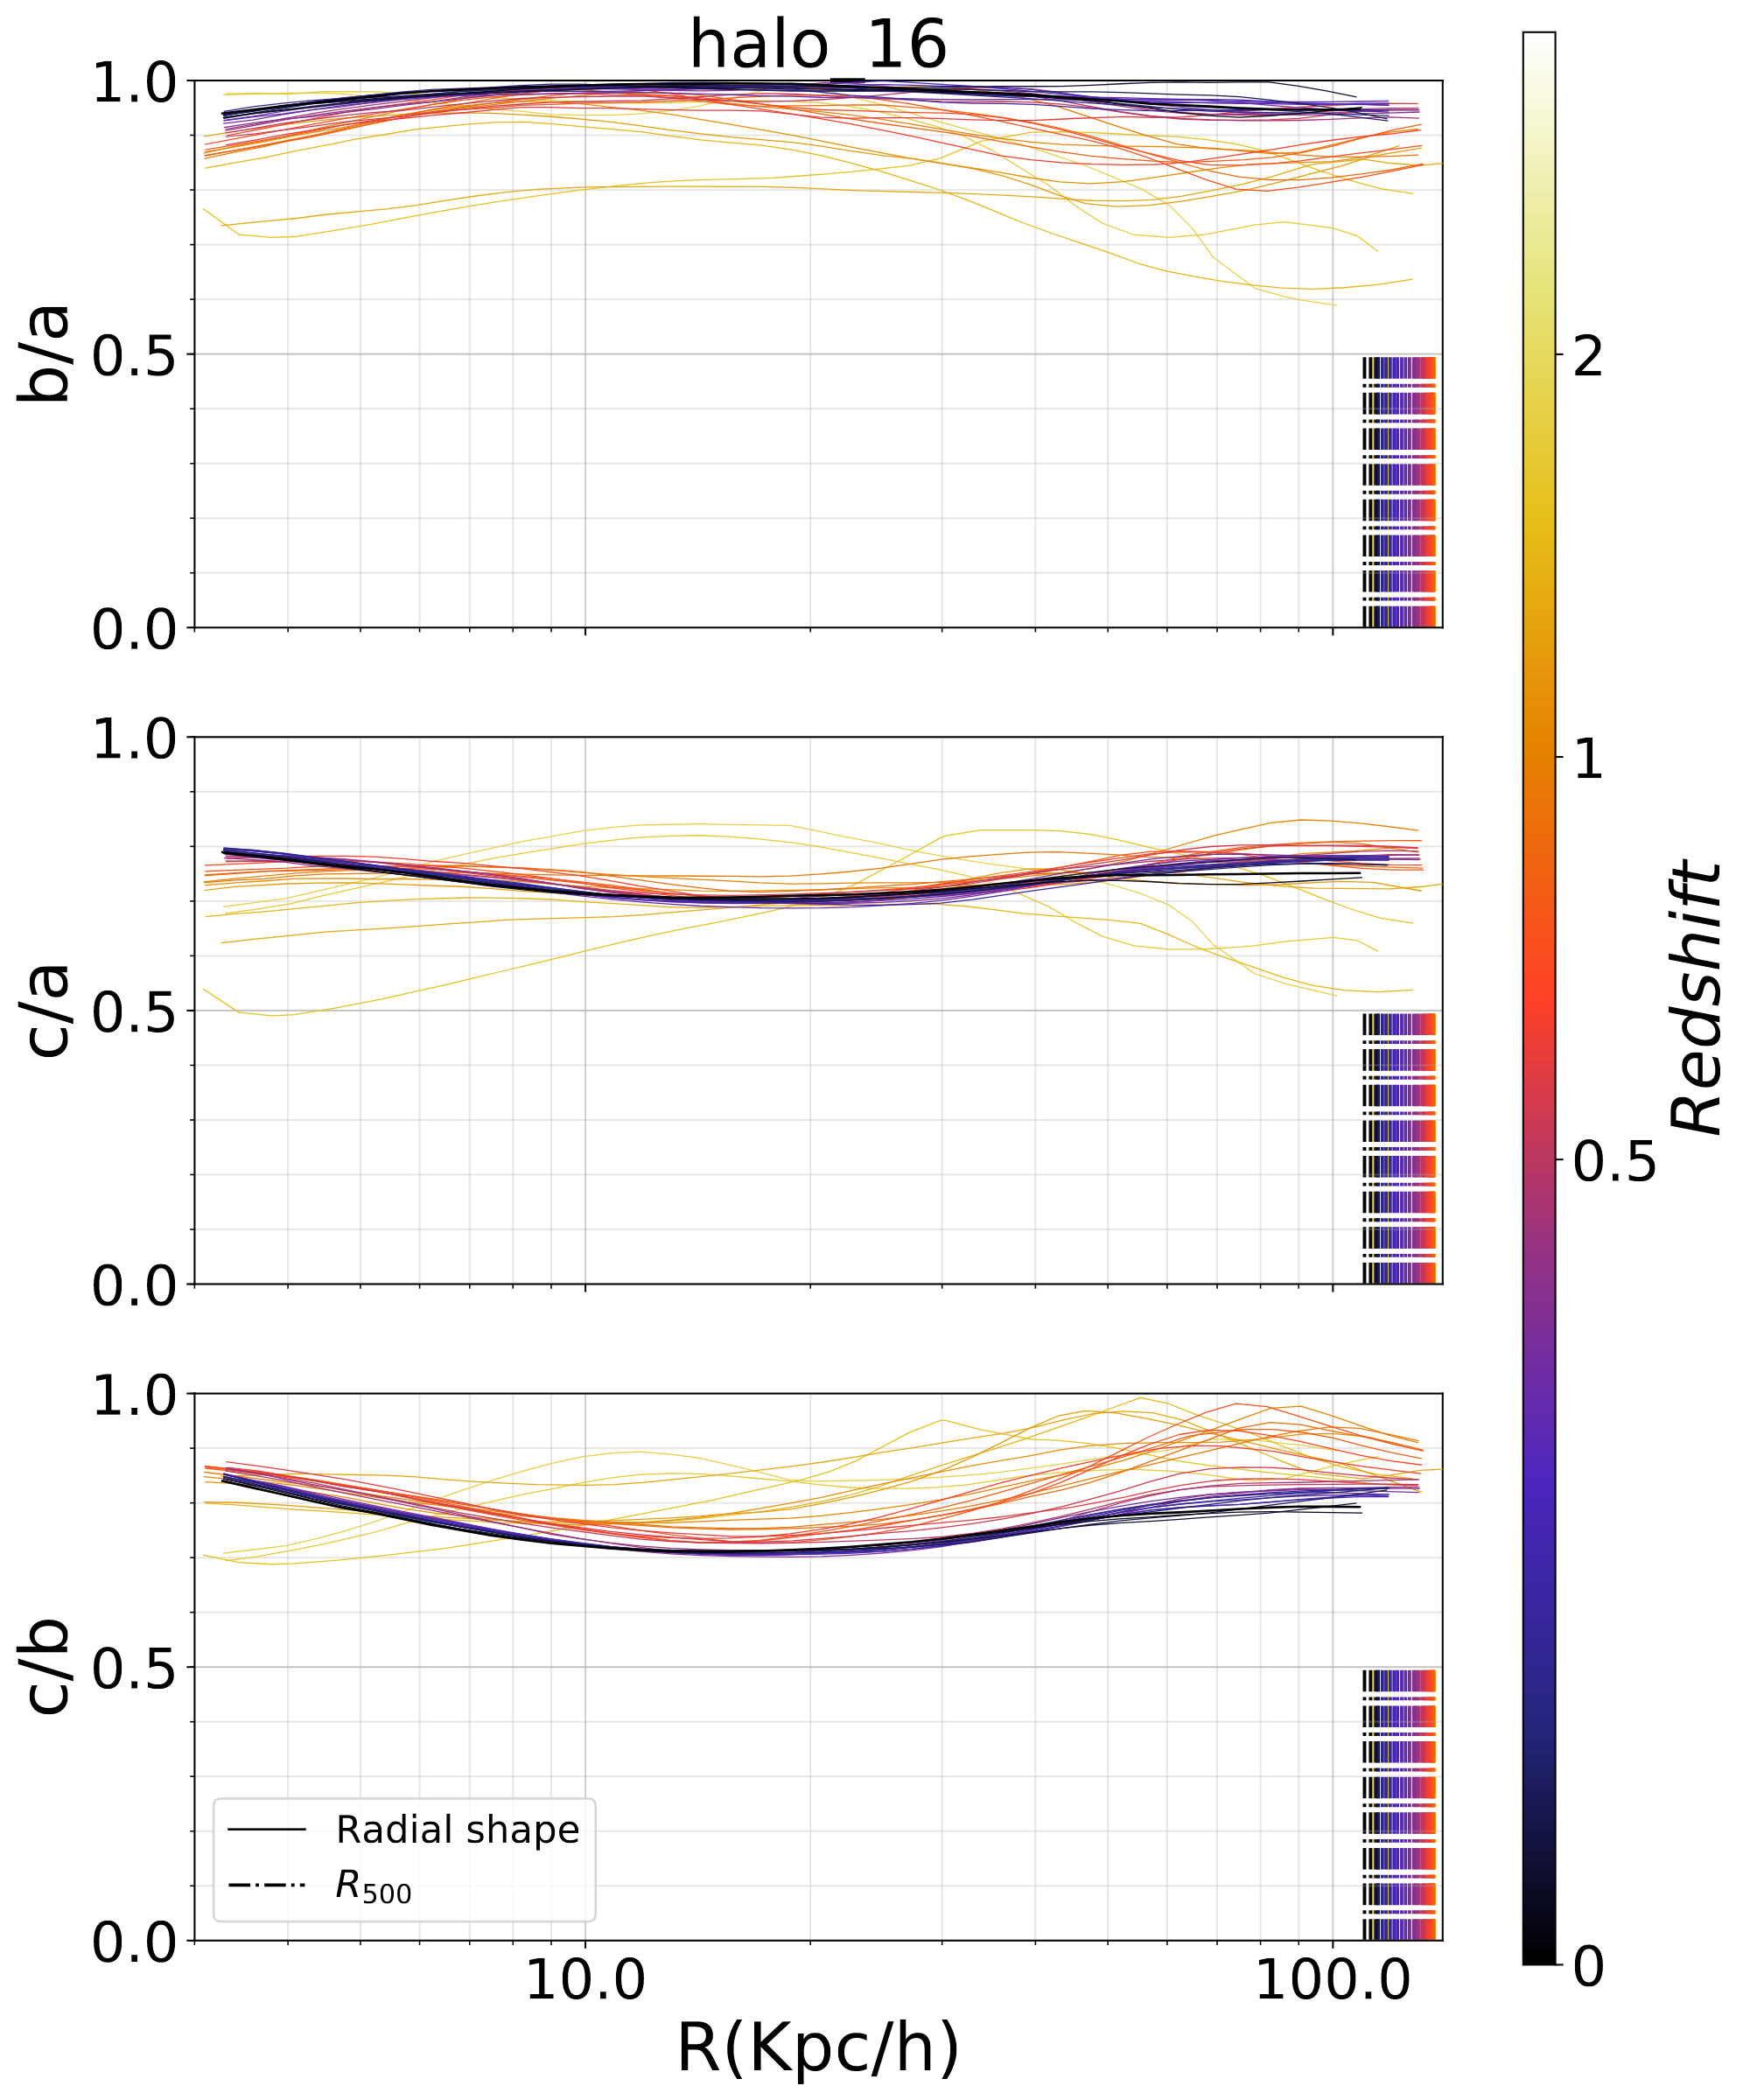
\includegraphics[width=0.5\columnwidth]{./pics/Redshift/halo_16_level3_MHD_Z.png}\label{fig:RedshiftMHDgood}}
  \caption{Example of historic shape conservation in comoving coordinates.\textbf{improve colorbar}}
\end{figure}


\begin{figure}[!ht]
  \centering
  \subfloat[halo 21 DM]{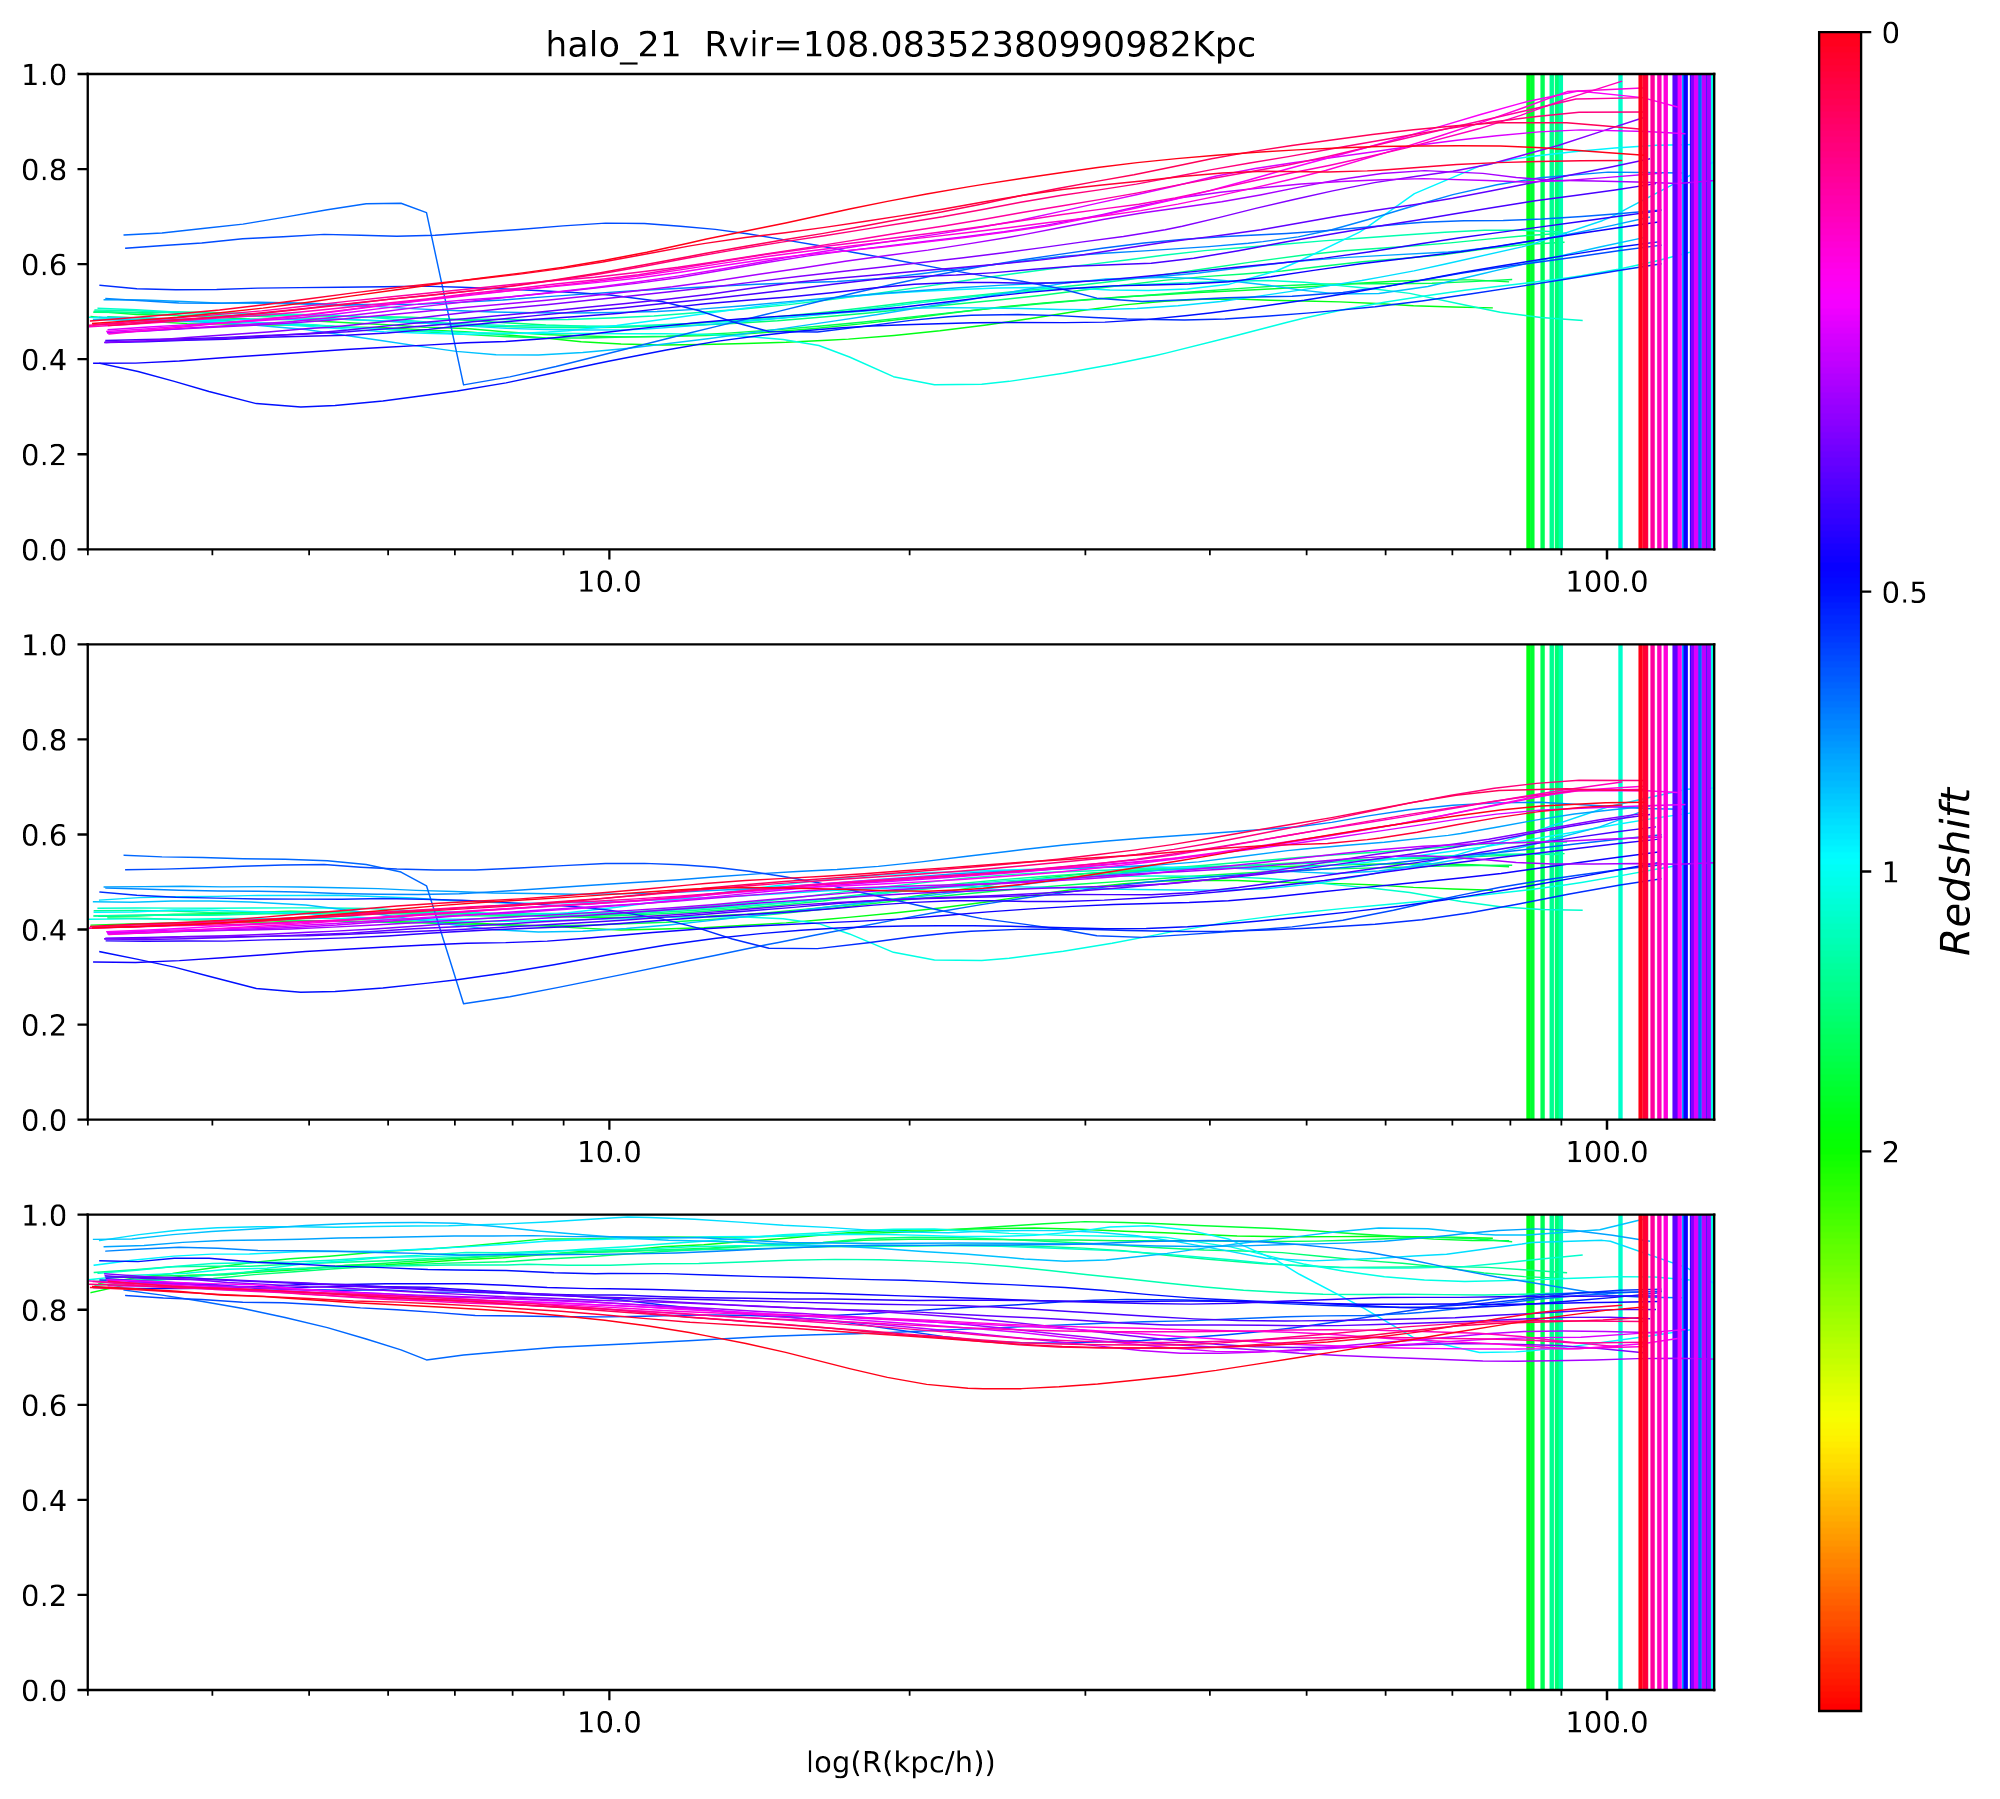
\includegraphics[width=0.5\columnwidth]{./pics/Redshift/halo_21_level3_DM_Z.png}\label{fig:RedshiftDMbad}}
  \hfill
  \subfloat[halo 21 MHD]{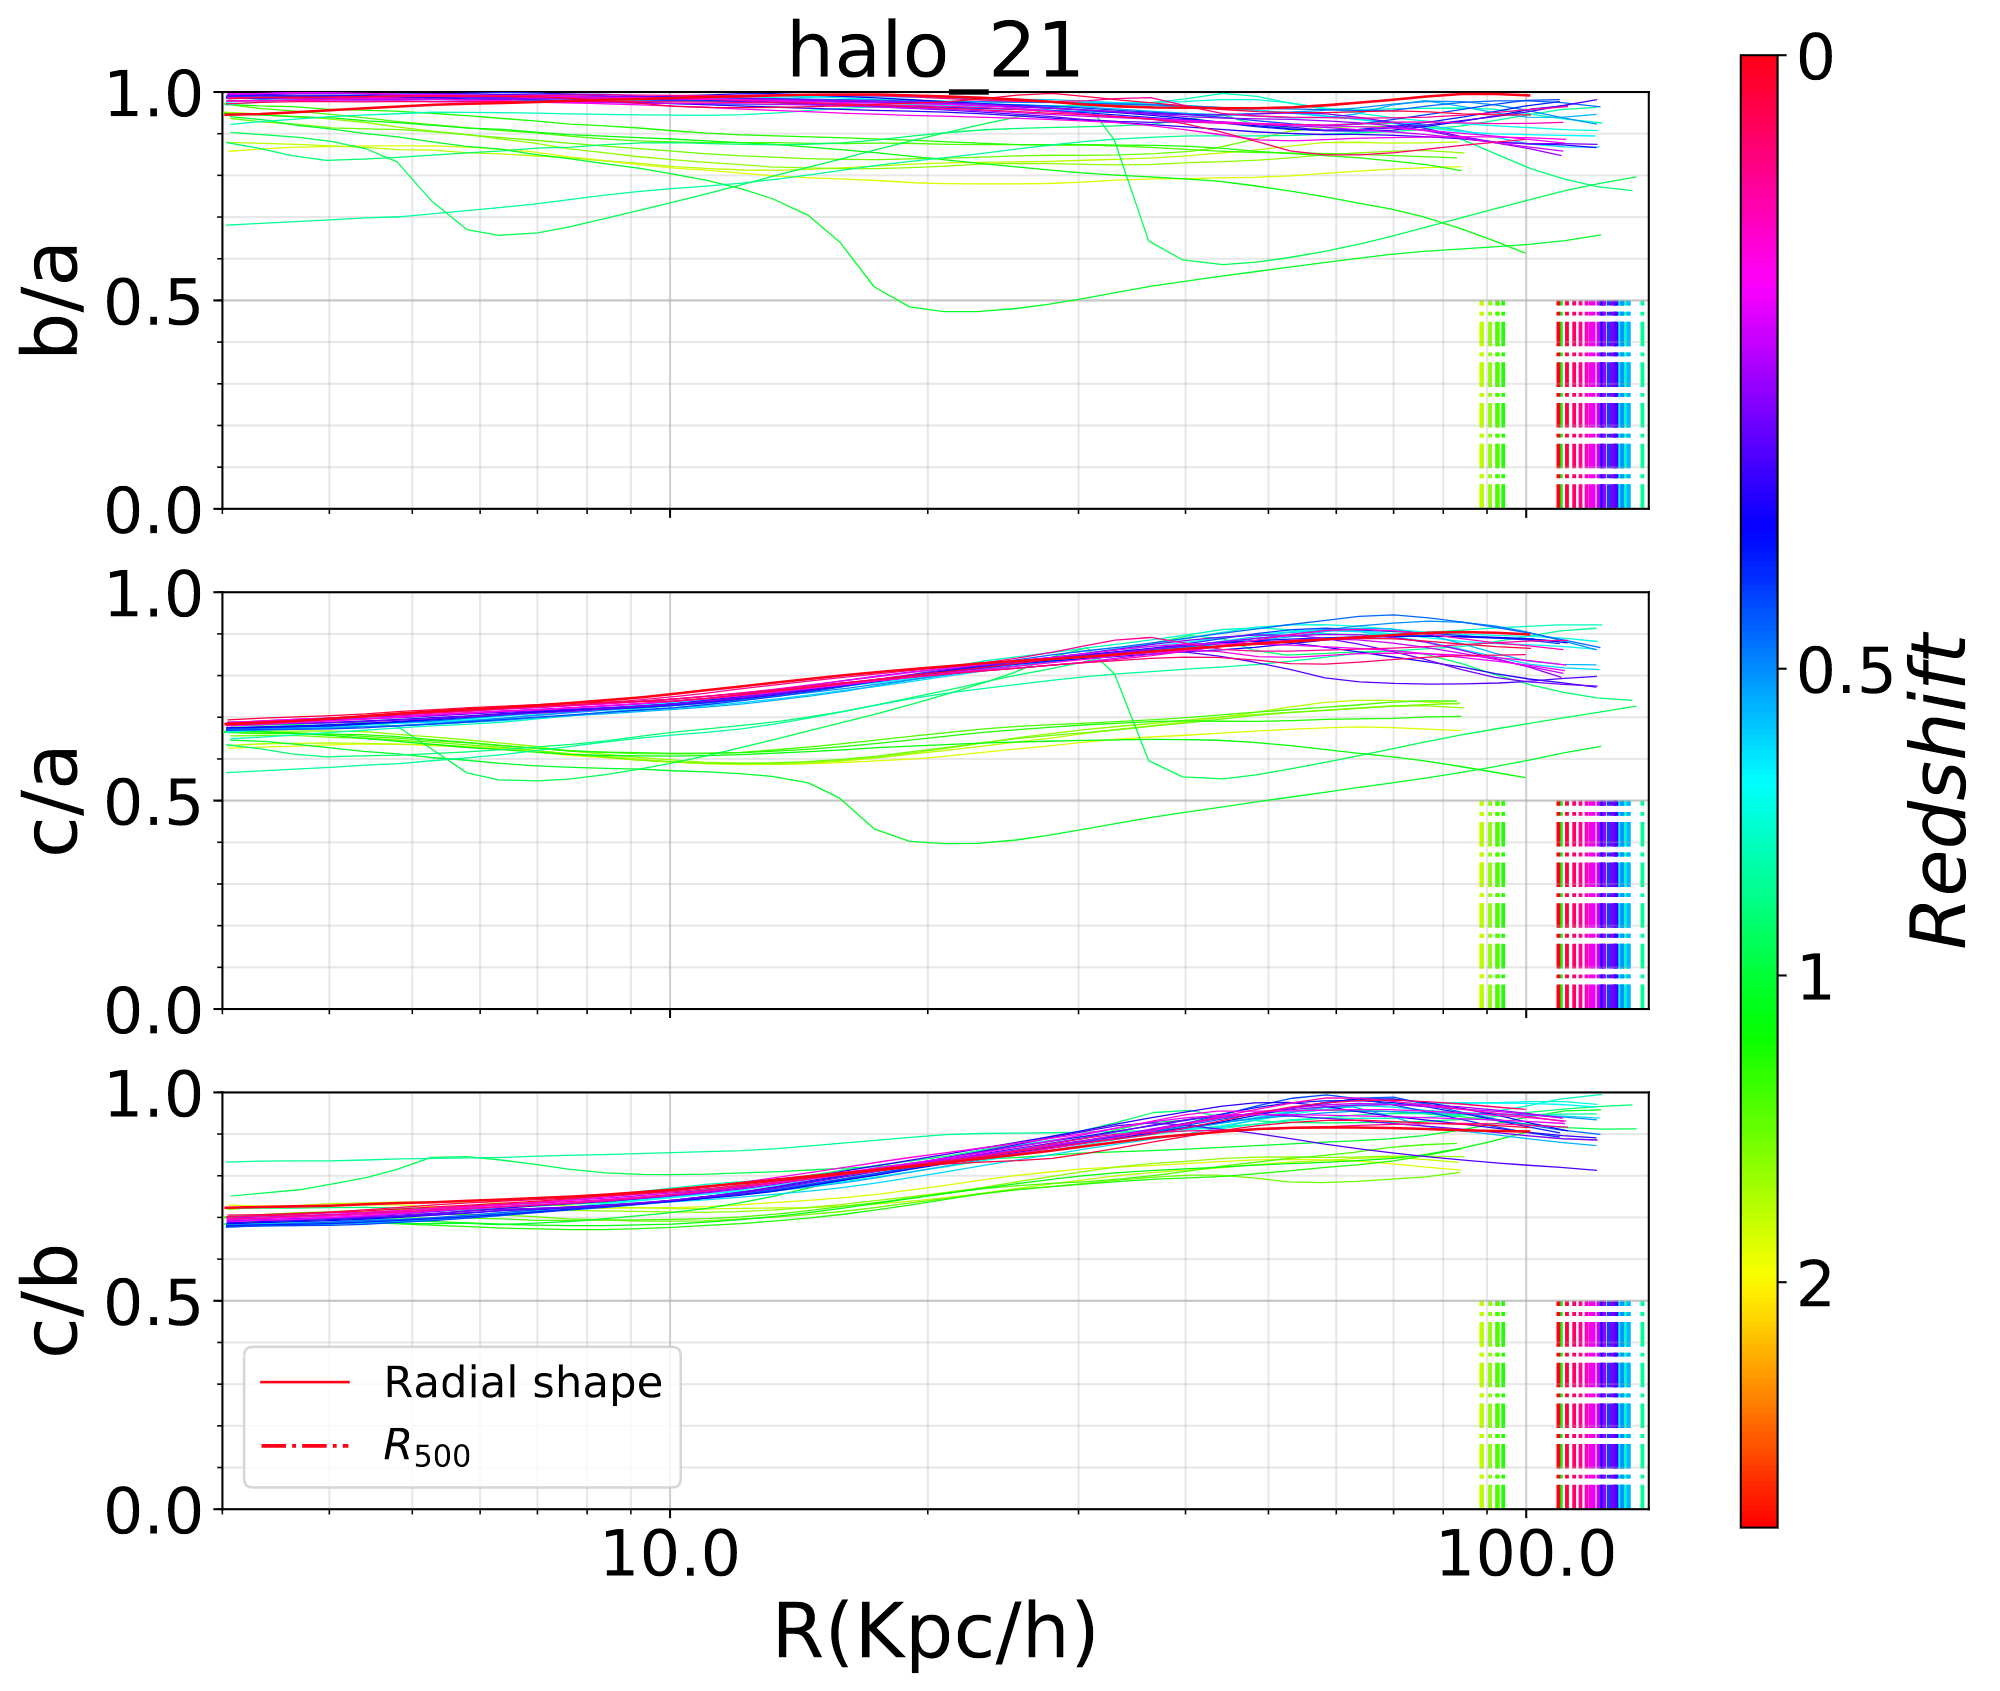
\includegraphics[width=0.5\columnwidth]{./pics/Redshift/halo_21_level3_MHD_Z.png}\label{fig:RedshiftMHDbad}}
  \caption{Example of historic shape disruption in comoving coordinates. The consistency between MHD and DM implies some major-event like a close merger or a collision. The non-continuous red line corresponds to the exact moment of this merging event, which is amplified in MHD.  \textbf{improve colorbar}}
\end{figure}

\begin{figure}[!ht]
  \centering
  \subfloat[halo 16 MHD]{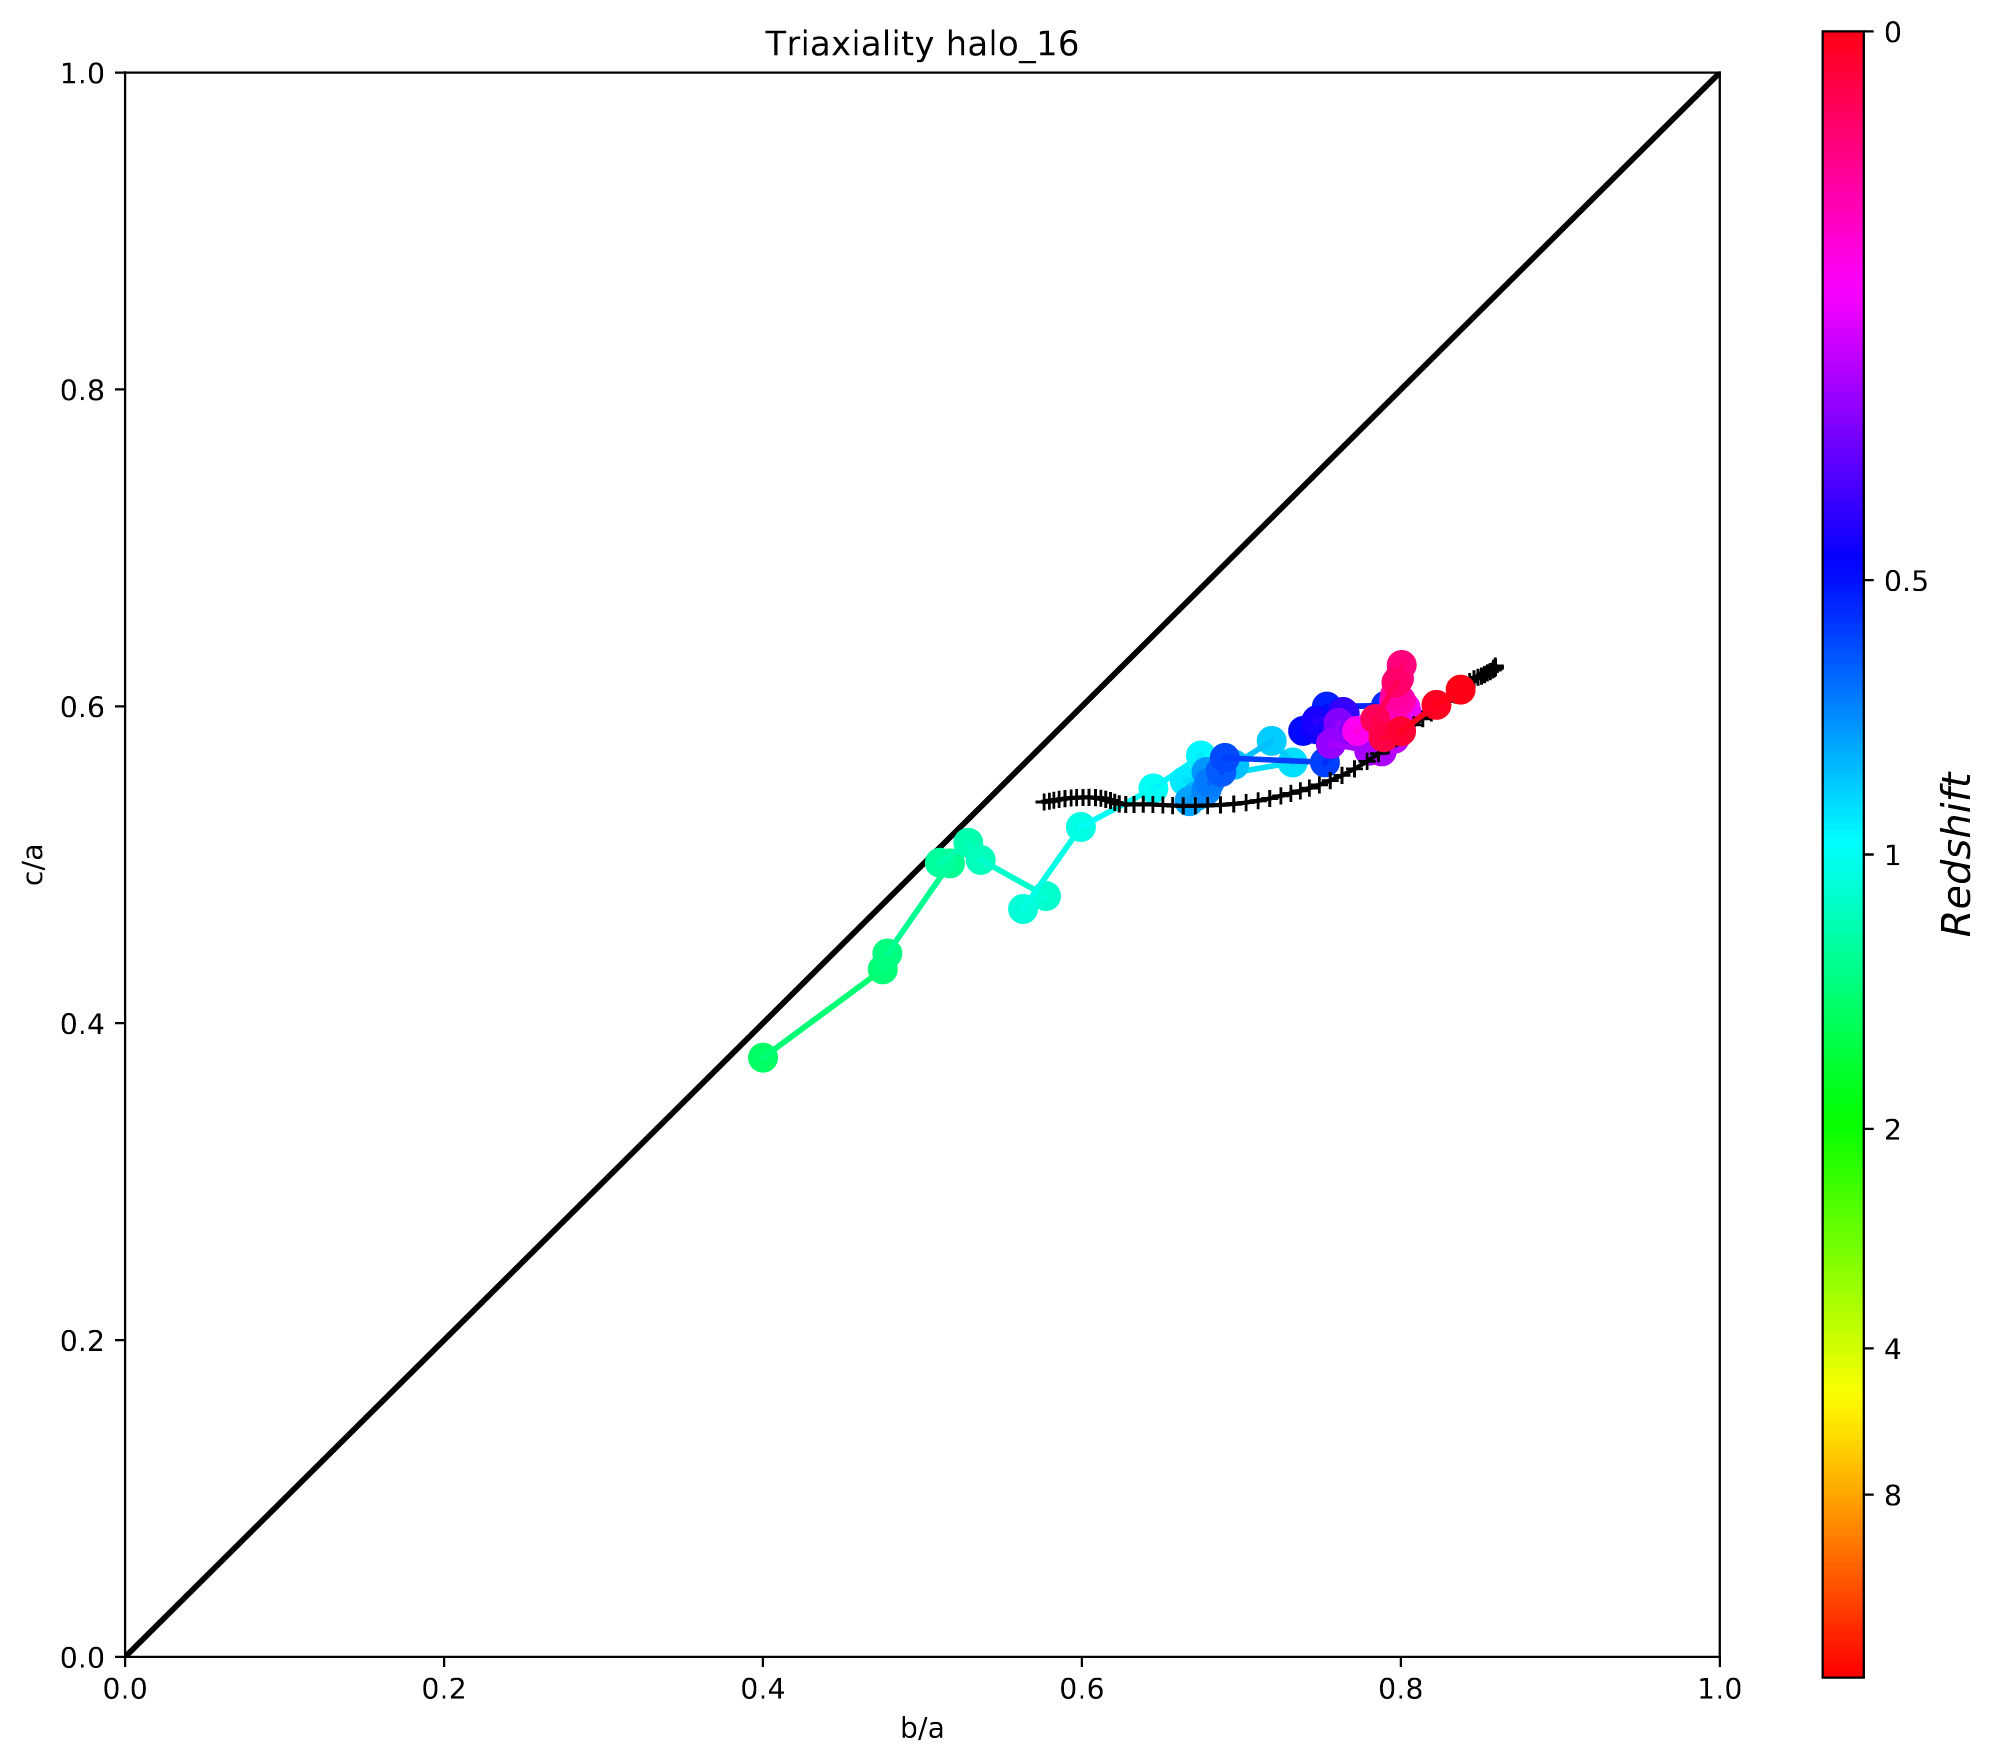
\includegraphics[width=0.5\columnwidth]{./pics/Redshift/halo_16_level3_MHD_Z_Triax.png}\label{fig:RedshiftDMTriax16}}
  \hfill
  \subfloat[halo 21 MHD]{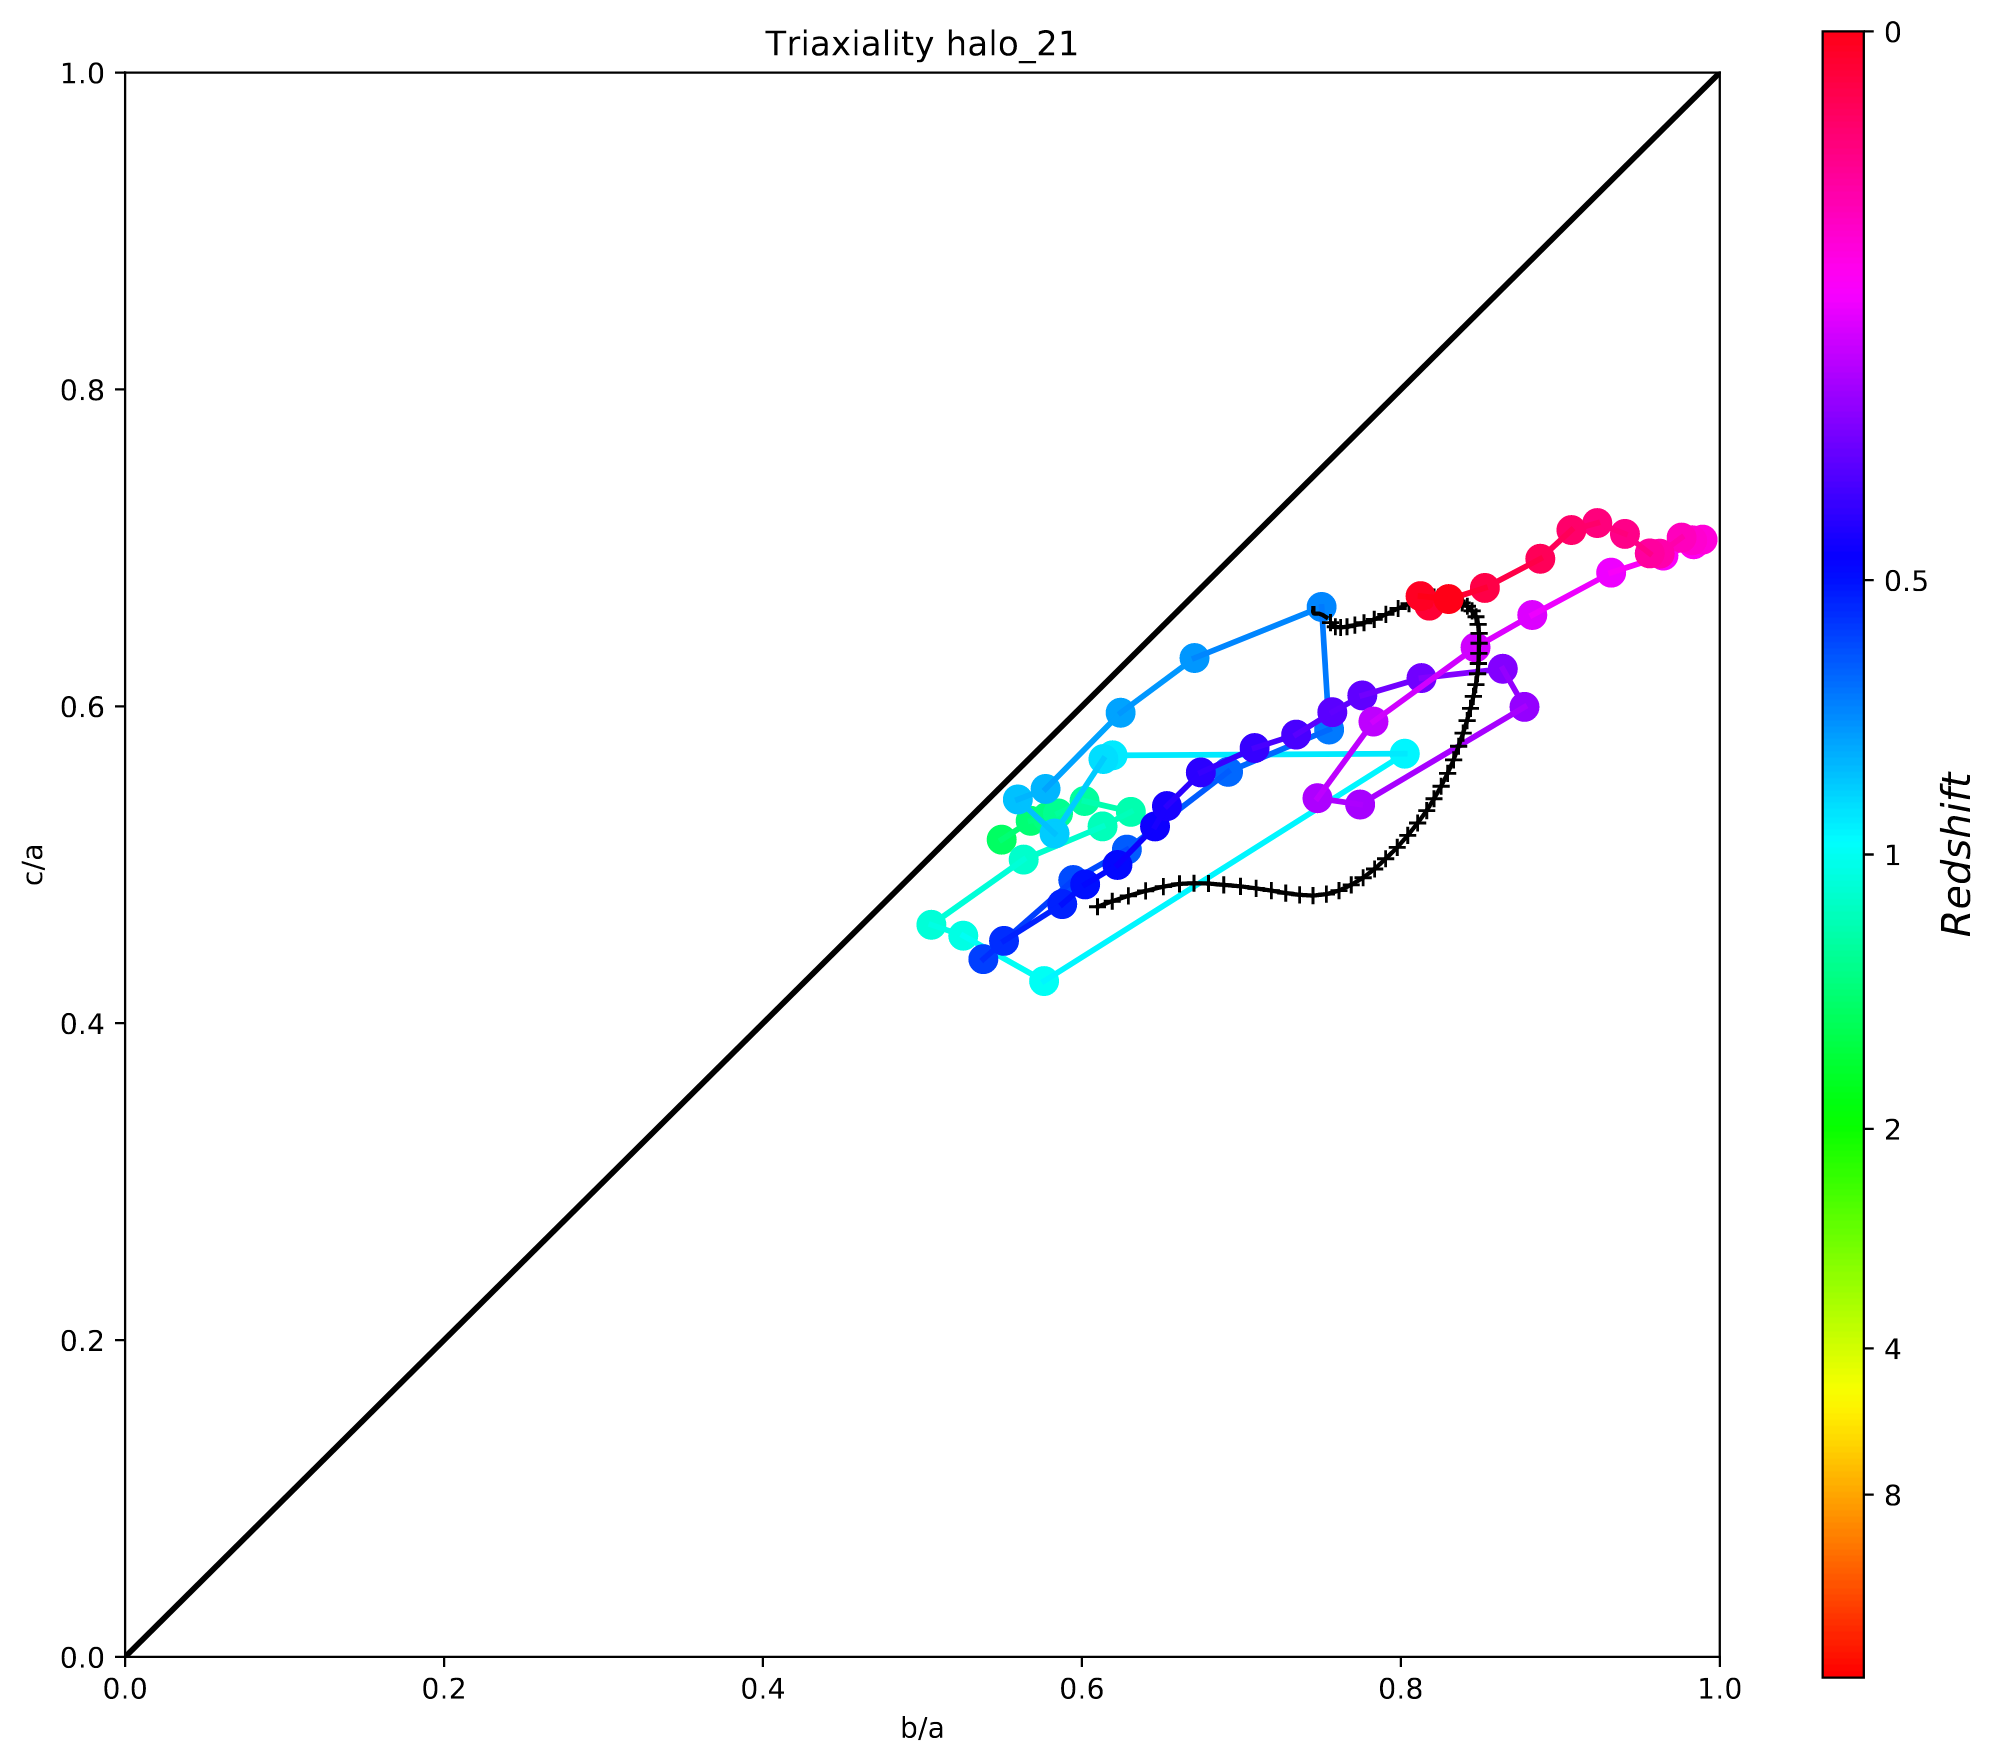
\includegraphics[width=0.5\columnwidth]{./pics/Redshift/halo_21_level3_MHD_Z_Triax.png}\label{fig:RedshiftDMTriax21}}
  \caption{Historic shape Vs radial shape on the Triaxiality plane. The black line represents the radial profile at redshift 0. The colored connected dots represent the shape measured at the virial radius (physical coordinates) at a certain redshift (color)}
\end{figure}




\end{figure}


 
